\documentclass[tocnopagenum]{thesis-ekf}
%a4paper, 12pt, 1.5-es sortávolság, margók
\usepackage[T1]{fontenc}
\PassOptionsToPackage{defaults=hu-min}{magyar.ldf}
\usepackage[magyar]{babel}
\usepackage{mathtools,amssymb,amsthm,pdfpages}
\footnotestyle{rule=fourth}
\usepackage{comment}
\usepackage{enumitem}
\usepackage{colortbl}
\newtheorem{tetel}{Tétel}[chapter]
\theoremstyle{definition}
\newtheorem{definicio}[tetel]{Definíció}
\theoremstyle{remark}
\newtheorem{megjegyzes}[tetel]{Megjegyzés}
\graphicspath{{./images/}}
\DeclareGraphicsExtensions{.png,.jpg,.pdf}
%excel to latex
\usepackage{booktabs}
\usepackage{bigstrut}

%algorithm
\usepackage{algorithm}
\usepackage{algpseudocode}


\begin{document}
	\institute{Matematikai és Informatikai Intézet}
	\title{Informatikai eszközökkel támogatott sport és egészségfejlesztés}
	\author{Sipos Levente\\Szak: Programtervező informatikus BSc\\Specializáció: Szoftverfejlesztő informatikus}
	\supervisor{Dr. Király Roland\\ egyetemi docens}
	\city{Eger}
	\date{2022}
	\begin{titlepage}
		\maketitle
	\end{titlepage}	
	\tableofcontents
	\begin{comment}
		leírom hogy miről szól, (nem kötelező), 2 rész -> probléma felvetés, mi a motiváció, kontextus, előremutatva a dolgozatban hol miről fogsz beszélni.(1.fejezetben befogom mutatni a kódolást)
	\end{comment}
	\chapter{Bevezetés}
	\par
	A tanulmányaim során sok olyan tantárgyat tanulhattam, amelyek segítettek bepillantást nyerni, abba, hogy melyik is az a terület az informatikán belül, amely felkeltheti érdeklődésemet. Az elmúlt évben tanulhattam robotikát, a \textbf{Robotika alapjai} nevezetű tárgy jóvoltából, amely közelebb vitt engem a hardver közeli programozás világába. Továbbá C\# nyelvben biztos tudást szerezhettem a \textbf{Szolgáltatás Orientált Programozás, Magasszintű programozási nyelvek I. és II.} című tárgyakban.
	\par
	Szakdolgozatom tematikájául egy olyan témát választottam, amely a későbbiekben mások számára hasznos lehet az informatikai tudás elsajátításában és alkalmazásában.
	Alapvetően mint keresztény hívő ember, úgy gondolom, hogy az emberi létünk egyik fő feladata és mozgatórúgója az, hogy segítsünk embertársainkon azokkal a technikákkal és tudásokkal, amelyek számunkra megadattak. Ezért örömmel tölt el az a lehetőség, hogy tanulmányaimat ennek megvalósítására fordíthatom.\\
	 "... a ti hitetek mellé ragasszatok jó cselekedetet, a jó cselekedet mellé tudományt..." (Biblia) 2 Péter 1:5
	\par
	A választott téma, mind az informatika mind az egészségügy számára fontos kérdéseket vethet fel:
	\begin{itemize}
		\item  Mi jelenthet arra megoldást, ha az idős korosztályba tartozó ember, aki nehézségekkel küzd a mindennapokban? 
		\item Tájékozódását, mozgását illetve kommunikációját hang, szín impulzusokkal összekapcsolva tudjuk-e hatékonyan segíteni az eszköz alkalmazásával?
		\item  Az informatikával tudunk-e az előbb említett kérdésre, olyan alkalmazást írni, amely segítségével a mozgásfejlődést elősegítheti?
		\item A testnevelés tudomány, az informatikával társítva, gyorsaságfejlesztésre, hogyan tudja hatékonyan bevetni a program által fejlesztett eszközt?
		\item Amennyiben tudunk erre alkalmas programot írni, hogyan valósítsuk meg gyakorlati és elméleti szinten?
	\end{itemize}
 	Ezen kérdések alapján keresem a válaszokat arra nézve, hogy az informatika hogyan tud segítségére lenni a rászorult és egészséges embereknek egyaránt. 
 
	Meglátásom szerint, ez egy hiánypótló kutatási téma, amely az embereknek a mozgását, és fizikai jólétét segítheti elő.
	Ezen eszközök leptikus területeket érintenek, vizuális illetve akusztikus hatások közreműködésével.
	\\
	A projekt fontossága az, hogy ezen eszközök segítséget tudjanak nyújtani, esetleg kiváltsák a beszédnek a szükségét. Beszéd helyett ezen eszközök segíthetik a mozgásában és tájékozódásban fejlődésre szoruló egyéneket. Mind a gyermekkortól az idős korig egyaránt eszköz lehet az egészségi vagy mentális érintettséggel küzdő embereknek.
	\par
	A digitális fejlődéssel arányosan egyre több eszköz nyújt segítséget az arra rászorulóknak, szakembereken keresztül. Jó példa erre a kutatásban lévő gondosóra, program amely a szociális segítésben vesz részt az idős gondozásban. A gondosóra biztonságot nyújt az idős ember és a hozzátartozói számára, mivel érzékeli ez az eszköz az esetleges testhelyzetváltozást, vitális paramétereket(Például: pulzus). A gondosóra mint ahogy a nevéből is adódik a technika segítségével egyfajta további felügyeletet biztosít.\cite{MTI}
	\par
	Ezen kívül kutatásom során még találkoztam a szakdolgozatom témájához hasonló másik projekttel is, amely a zene és a dallamok együttes hatását, mint egy "segédeszközt" használ fel, amelyet szaknyelven "Zeneterápiának" hívnak.\cite{zsofia2021zeneterapia}
	\\
	Az erről szóló cikk, "A zeneterápia útjai: Traumától az újratanuláson keresztül az inklúzióig" 2.1-es fejezet 2.1.1 "Zeneterápia" című alfejezetében így ír a szerző:
	„Zeneterápia során a képzett zeneterapeuta egy tervezett folyamatban használja a zenét vagy a zenei elemeket (hang, ritmus, dallam, harmónia) annak érdekében, hogy elősegítse a kommunikációt, kapcsolatokat, tanulást, kifejezést, mobilizációt, szervezést, szerveződést."
	\par
	Továbbá, egy másik módszer alapján Erdélyi Ilona arról ír, hogy az érett korúak számára létrehoztak egy emlékeztető szobát amelyben a demens betegek, fiatal korukban használt tárgyaik segítségével emlékezhettek vissza életük korai szakaszára. Ezen memóriaterápia segíti előhozni emlékeiket, és általános jólétüket javítja.\cite{erdelyiilonademensbetegek}
	
	A szakdolgozatom célja, egy olyan program kidolgozása és megvalósítása ami az embereknek, a fizikai, és mentális állapotának stabilizálásában, és fejlesztésében eszköz lehessen.
	\par 
	
	A következő fejezetekben azt fejtem ki, hogy milyen technológiákat használunk, és emellett milyen programozási nyelven készül el. \\ 

	
	\begin{comment}
	Bevezető2: Rendszer amit kidolgozott Somodi László, mi a szerepe, mi a célja, mit vállaltam én? -> frontend
	\end{comment}
	\chapter{Szakdolgozatom elméleti alapjai}
	\section{Háttérelméleti forrás}
	\par
	A témában jártas, és a "Mozgáskoordináció- és gyorsaságfejlesztő gyakorlatok óvodától a felnőtt korig" \cite{SLaszlo} című könyv, melynek írója, Somodi László, segített betekintést nyerni az egészségügyi és a morális hátterébe a projektnek. \\ Elmondása szerint a mozgásfejlesztés és az agyi kapacitás fejlesztése, kéz a kézben jár. Ezt a fejlesztést úgy érhetjük el, ha az adott személynek utasításokat adunk ki, hogy adott jelzésre (szín, hang, irány) és ezek kombinációjára, milyen mozgást kell végeznie.
	\par 
	\subsection{Gyakorlati haszna}
	Az agy mentális funkcióinak erősítése, speciális koordinációfejlesztő gyakorlatokkal is lehetséges melynek a három komponense a következő: 
	\begin{enumerate}
	 
			\item	Az első komponens a koncepció, vagyis az a módszer, ami alapján a rendszer elkészült. A koncepció egészségügyi, és sport-rekreációs tevékenység alapú.
			\item	A második komponens a hardver, ami a mozgáshoz és a gyakorláshoz szükséges időzítést, jelzéseket adja, és vezérli az aktivitást, amit a koncepció előír.
			\item	A harmadik komponens a hardvert meghajtó, és így a feladatokat közvetlenül irányító, programozható, tanítható szoftver.
	\end{enumerate}
	\subsection{Módszer létfontossága}
	Az a személy aki használja ezt a módszert, nála külön dolgozik a két kar, külön dolgozik a két láb és ezáltal folyamatosan kapcsoljuk át a két agyféltekét.
	Továbbá, a könnyen és egyszerűen felismerhető hang, szín, és ábra jelzések az esetlegesen a fogyatékossággal élő emberek számára is érhető és a jelzések értelmezése nem jelenthet akadályt.
	\\
	Különféle álló helyzetek (alapállás, mellső középtartás, magas tartás) képesek segíteni abban, hogy az idegpályákon lévő átkapcsolódási pontok (szinapszisok) száma növekedjen. Fiatalabb korban a szinapszisok számát, későbbiekben az átkapcsolódási pontok erejét növeli.
	Sokféle betegség felmerülhet az olyan embereknél akiknek ez a módszer alkalmas lehet, a könnyen felismerhető és megérthető eszközök.
	Továbbá, ez által a módszer által gyorsabban megértjük az elvégzendő  feladatot, feladatokat és akár gyorsabban is végrehajthatjuk azokat.
	  %szellemi leépüléssel küzdő, szép korúak számára is segítséget nyújthat, mivel a változatos mozgás, és a különböző ingerek ki- és be- kapcsolása növeli az agy alap működését.
	 \\
	Elméletből következhet az, hogy a módszer hasznosan alkalmazható általános, és akár hátrányos helyzetű gyerekeknél és felnőtteknél is egyaránt.
	A módszert kis helyen és minden korosztálynál lehet alkalmazni, de a teljesség érdekében, a módszer intelligens szobával együtt működik hatékonyan.
	
	
	\subsection{Intelligens szoba röviden}
	Az intelligens szoba kifejezés egy olyan helység, melynek mind a négy falán, vagy oldalán különböző jeladókat helyezünk el.
	Ezek különböző eszközök melyek típusai lehetnek: fények, színek, nyilak és hangok. Ezek külön, vagy együttesen kiküldött jeleire különböző, illetve speciális koordinációfejlesztő feladatokat végrehajtani. Minden egyes különböző szín, és fényjelzés, más és más feladatokat tartalmaznak.
	Ez azt jelenti, hogy adott esetben egy piros lámpa színe emlékeztethet arra, hogy a piros szín jelentése szimbolikus hatással bír.Melyet az adott ember köthet a már mindennapos életben tapasztaltakhoz. Nyilak felvillanására, különböző hangokra pedig más érzékeket váltunk ki mint például a fényjelzés esetén. Ilyenkor irányváltásokat kell végrehajtani amik máris komplikálják egy kicsit az adott mozdulatokat.
	\\
	Ezzel a módszerrel és az intelligens szobával együttesen tudjuk a mozgáson keresztül úgy stimulálni az agyat, hogy a legrövidebb idő alatt a legtöbbször átkapcsoljuk. (200-szor, 300-szor, 400-szor, stb.)
	\par
	\subsection{Automatizálási megoldások a programban}
	A fentebb említettek automatizálására készül a projekt, amely különböző informatikai eszközökkel valósítja meg a színek, hangok, és nyilak megjelenítését, illetve érzékeltetését. 
	A hardver komponensek. A hardver több egymáshoz tetszőlegesen kapcsolható smart box, amelyek közül van amely képes fényjelzések kiadására, továbbá van olyan eszköz is amely képes nyilakat képezni ábra szerűen, legutolsó sorban pedig az utolsó féle eszköz képes hangjelzések kiadására. A smart box-okat szoftveresen lehet vezérelni, így azok képesek a koncepció alapján összetett mozgások, vagy komplex feladatsorok irányítására.
	\begin{comment}
	Ennek egy példája a \pageref{table:egyedzesterv}. oldalon található táblázat amely az automatizálásra létrehozott "edzéstervet" mutat be.[\ref{table:egyedzesterv}]
	\end{comment}
	\\
	Alapvetően, a projekten több tudományágban ismerős, és érdekelt személy vett részt. 
	\\
	Ezek a személyek a következők:
	\begin{itemize}
		\item Elméleti háttér kidolgozásában és kutatásában, Somodi László UEFA "A" licences labdarúgó szakedző.
	
		\item A hardver lefejlesztését és összeszerelését, Keresztes Péter Tanár úr végezte . 
		\item A példaprogramot Delphi-ben, Dr. Király Roland Tanár úr fejlesztette le. 
		\item A back-end és ezeknek a hardvereknek a mögöttes működtetését, valamint a Delphi és a C\# nyelvek közötti kapcsolat megoldását, Nagy-Tóth Bence, barátom és szaktársam készítette el.
	\end{itemize}
	Én ezeknek a hardvereknek a működtetéséhez a felületet írtam, amin keresztül lehet különféle módon, vezérelni a fentebb említett eszközöket. %változatos ütemekben vezérelni a fentebb említett eszközöket.
	\\ 
	Ezt C\# nyelven írtam, ami egy friss és modern felhasználói felület írására és elkészítésére alkalmas.
	
	\chapter{Szakdolgozatom elaborálása}
	\section{A projekthez tartozó eszközök bemutatása}
	Háromféle eszközt szeretnénk működtetni, lámpákat, nyilakat, illetve hangszórókat. Az eszközöknek többféle bemeneti csatlakozói vannak, de ezekről a későbbi  \ref{eszkozcsatlakozok} alfejezetben található meg.
	Ezen eszközöket Keresztes Péter Tanár úr készítette, és szerelte össze.
	Továbbá, mindegyik eszköz más és más érzékszervet stimulál, mint például a lámpa színének a felvillanása a szemünkre van nagy hatással, míg a hangszóró a hallásunkat veszi igénybe. 
	\subsection{Lámpa eszköz}
	A lámpa eszköz egy olyan LED-ek összessége melyben a fény akkor keletkezik, amikor az áramot vezető részecskék egyesülnek a félvezető anyagban. Az eszköz képes különféle színek kibocsájtására is, melyek vezérlését a tervezett felületen keresztül lehet vezérelni.
	\begin{figure}[H]	
		\centering
		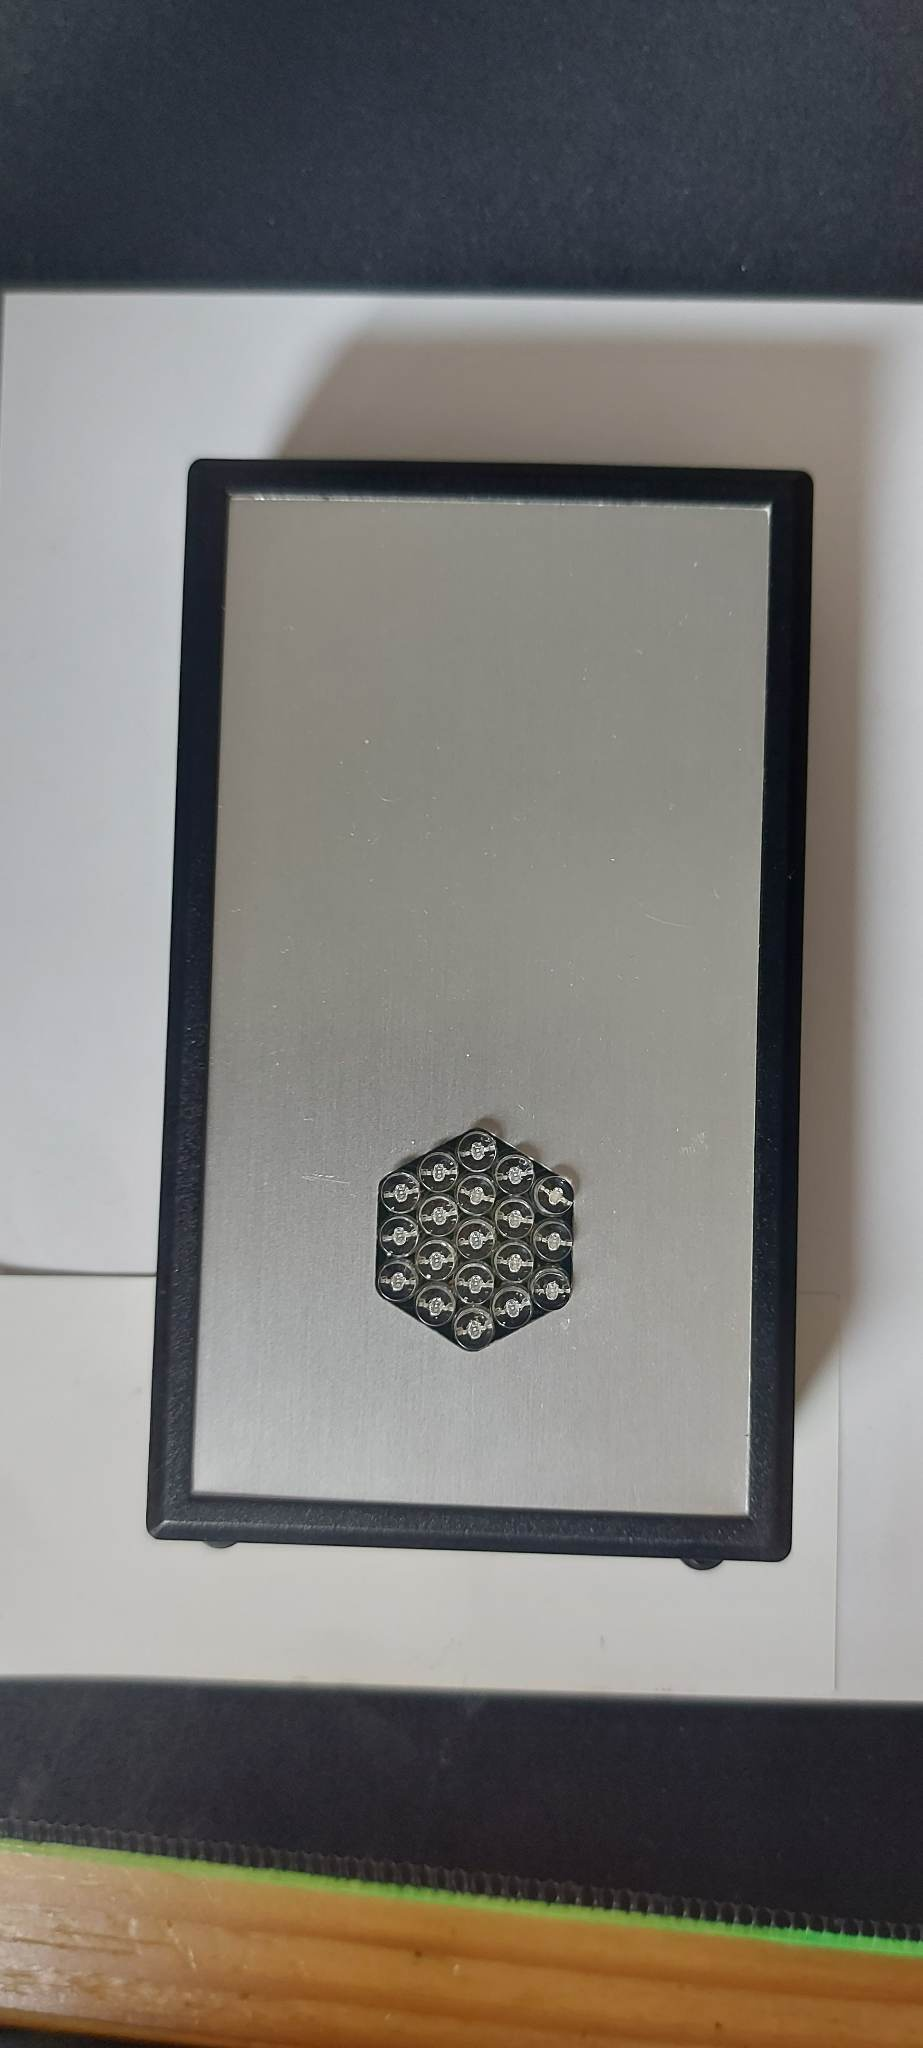
\includegraphics[scale=0.10]{lamp01}
		\caption[Lámpa eszköz]{Lámpa eszköz}
		\label{fig:lamp01}
	\end{figure}
	Ezen az eszközön összesen 19 db dióda található meg amelyek egységesen tudnak funkcionálni. 
	Az eszköz a \ref{fig:lamp01} ábrán látható.
	A lámpa eszközről készült videofelvétel is amelyről az alábbi \url{https://www.youtube.com/watch?v=szECXr9RMNQ} linken találhatunk felvételt.
	\subsubsection{Fénykibocsátó diódákról röviden}
	A LED félvezető anyagában vannak energiasávok, és ezek elkülönülése határozza meg a LED által kibocsátott fényrészecskék energiáját.
	Ezek a fényrészecskék határozzák meg a kibocsátott fény hullámhosszát, ezt követően a színét is. A nem megegyező sáv különbségek adják azt meg, hogy különféle színt eredményezzenek ezek a félvezető anyagok.\cite{leds_magazi}
	\subsection{Nyíl eszköz}
	A nyíl eszköz egy olyan eszköz amely különféle irányok megjelenítésére képes. Ezt úgy tudja elérni, hogy különböző sorrendben, más pozícióban éri az áram a diódát, ezzel elérve, hogy mintegy nyíl funkcionáljon.
	Az eszköz képes különféle színek kibocsájtására is, továbbá irányok jelzésére is alkalmas, melyek vezérlését a tervezett felületen keresztül lehet vezérelni. 
	Ezen az eszközön összesen 26 db dióda található meg amelyek egységesen is tudnak funkcionálni.	
	Maga az eszköz a \ref{fig:nyil01} képen látható.	\begin{figure}[H]	
		\centering
		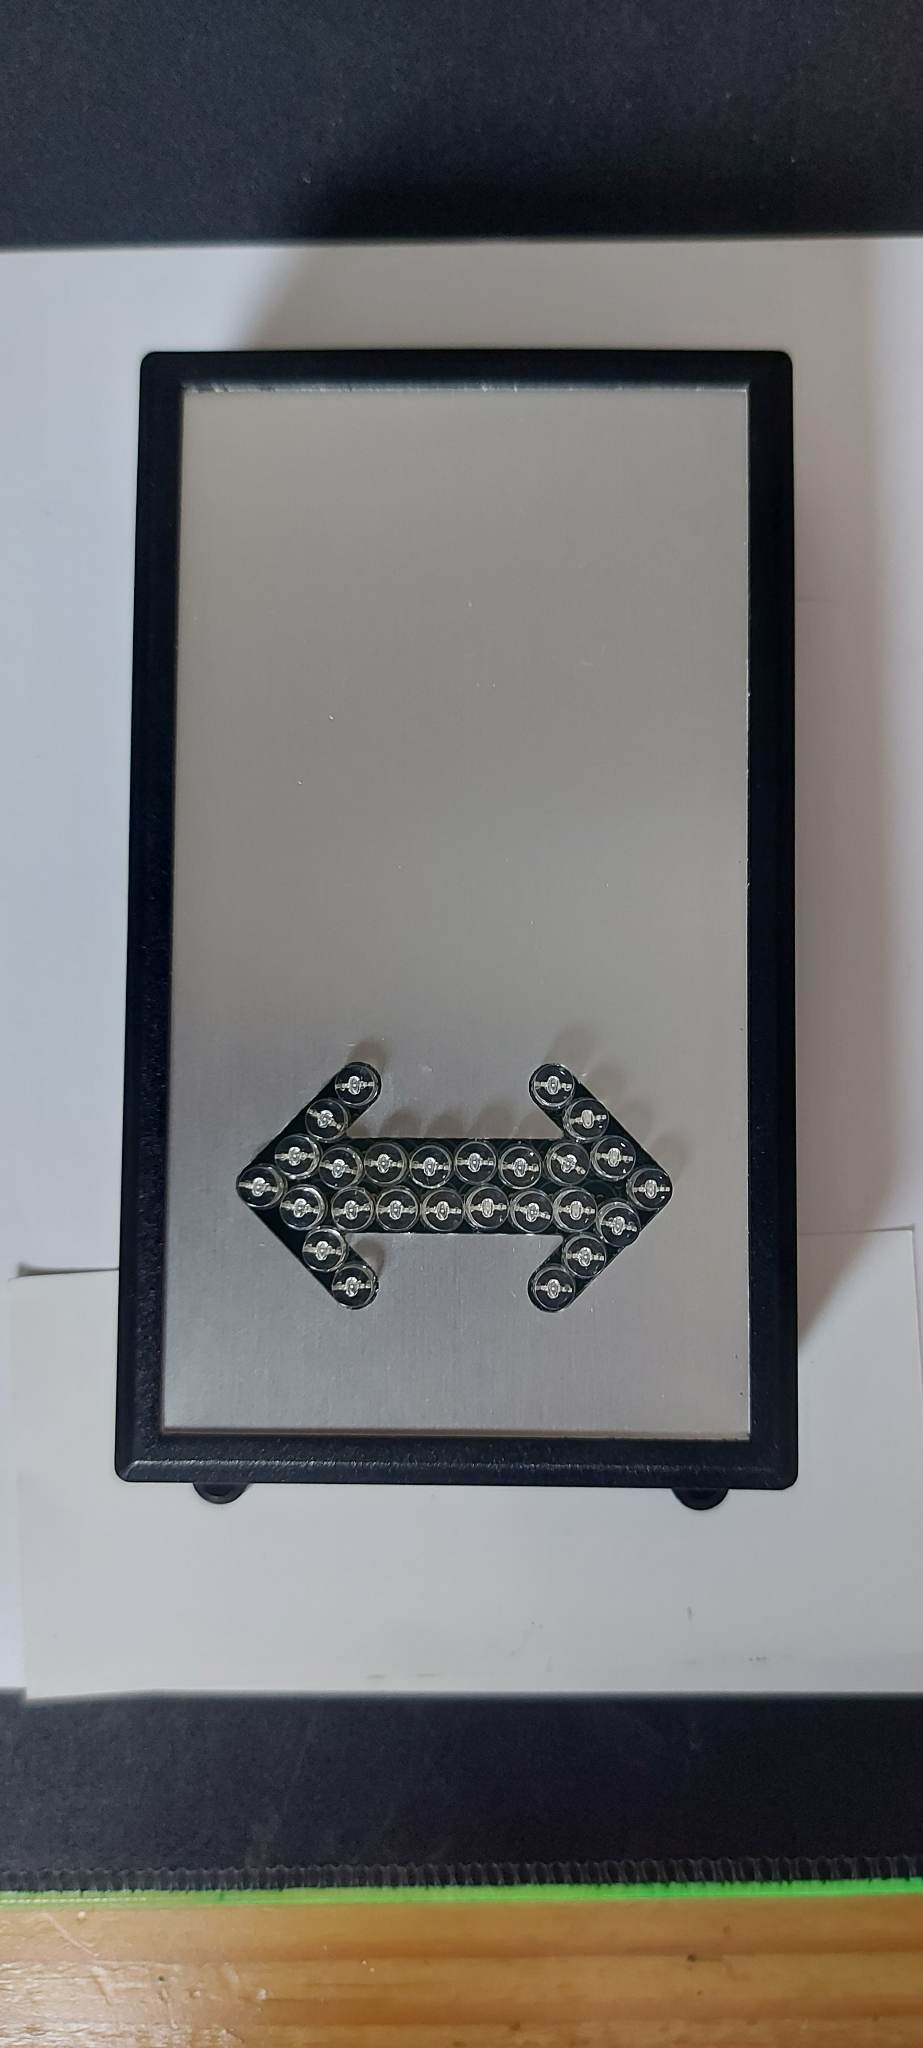
\includegraphics[scale=0.12]{nyil01}
		\caption[Nyíl eszköz]{Nyíl mint eszköz}
		\label{fig:nyil01}
	\end{figure}
A lámpa eszközről készült videofelvétel is amelyről az alábbi \url{https://youtu.be/shEyutbeBes} linken találhatunk felvételt.
\newpage
	\subsection{Hangszóró eszköz}
	A hangszóró, mint eszköz képes különféle hangszínen, más és más hangerőn hangokat lejátszani. Továbbá, egy hangszín lejátszásának a hosszát is betudjuk konfigurálni. Mind ezek alapvető funkcionálását és bekonfigurálását képesek vagyunk vezérelni a projekthez tartozó alkalmazással. A hangszóró emellett képes akár arra is hogy különböző hangszíneket lejátsszon egymást követően, ezzel akár különféle dallamokat és dalokat tudunk lejátszatni a hangszórónk segítségével.
	\\
	Magáról az eszközről a \ref{fig:hangsz01} ábrán találhatunk egy képet.
	\begin{figure}[H]	
		\centering
		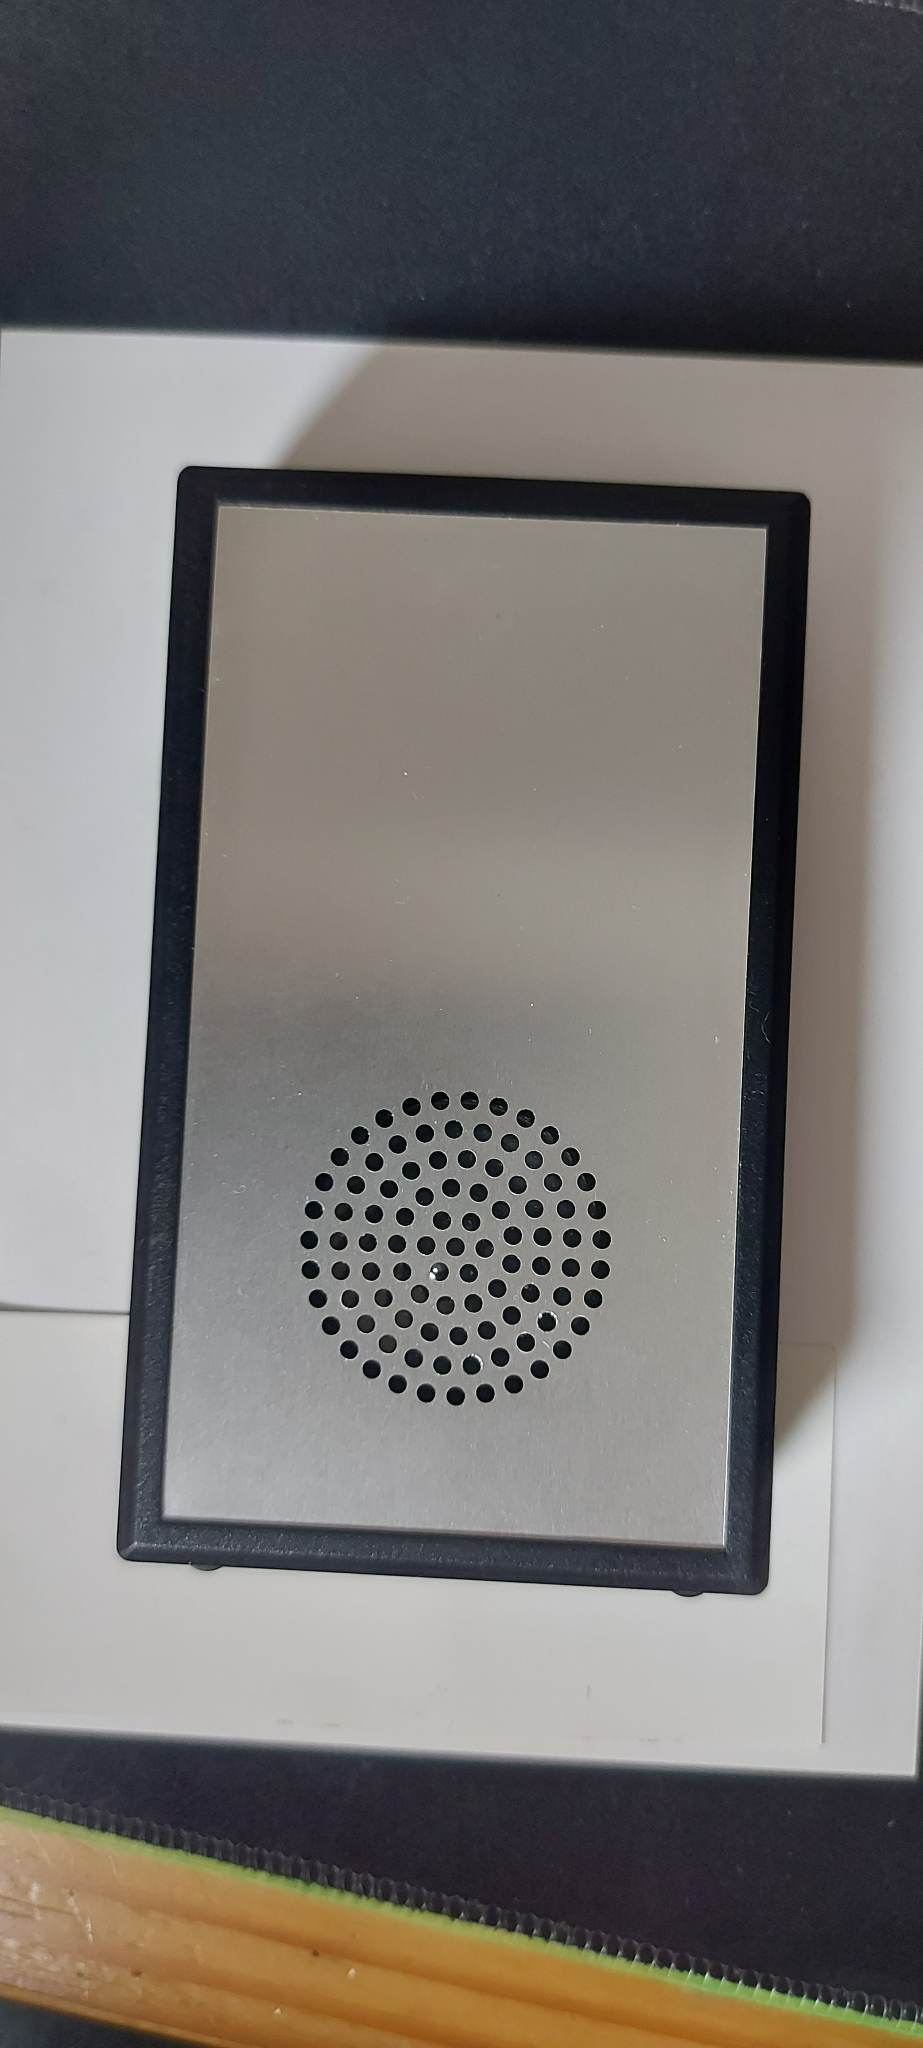
\includegraphics[scale=0.10]{hangsz01}
		\caption[Hangszóró eszköz]{Hangszóró eszköz}
		\label{fig:hangsz01}
	\end{figure}
A lámpa és a hangszóró eszközökről készült videofelvétel is amelyről az alábbi \url{https://youtu.be/shEyutbeBes} linken találhatunk felvételt.
	\subsection{Eszközök csatlakozói}
	\label{eszkozcsatlakozok}
	Ezen eszközöknek önálló tápellátással rendelkeznek, továbbá az eszközök közötti kapcsolatot, 4 pólusú RJ típusú csatlakozókkal felszerelt kábelen keresztül lehet biztosítani. Ezek közül is az RJ 9-es változatát használjuk amely egy 4 eres csatlakozó, amibe csak a középső kettő(piros,zöld) vezetékeket kötjük be.
	Az eszközök aljzatai mind egységesen vannak felépítve, ezen aljazatokról a \ref{fig:csatlakozo} ábrán találhatunk képet.
	\begin{figure}[h!]	
		\centering
		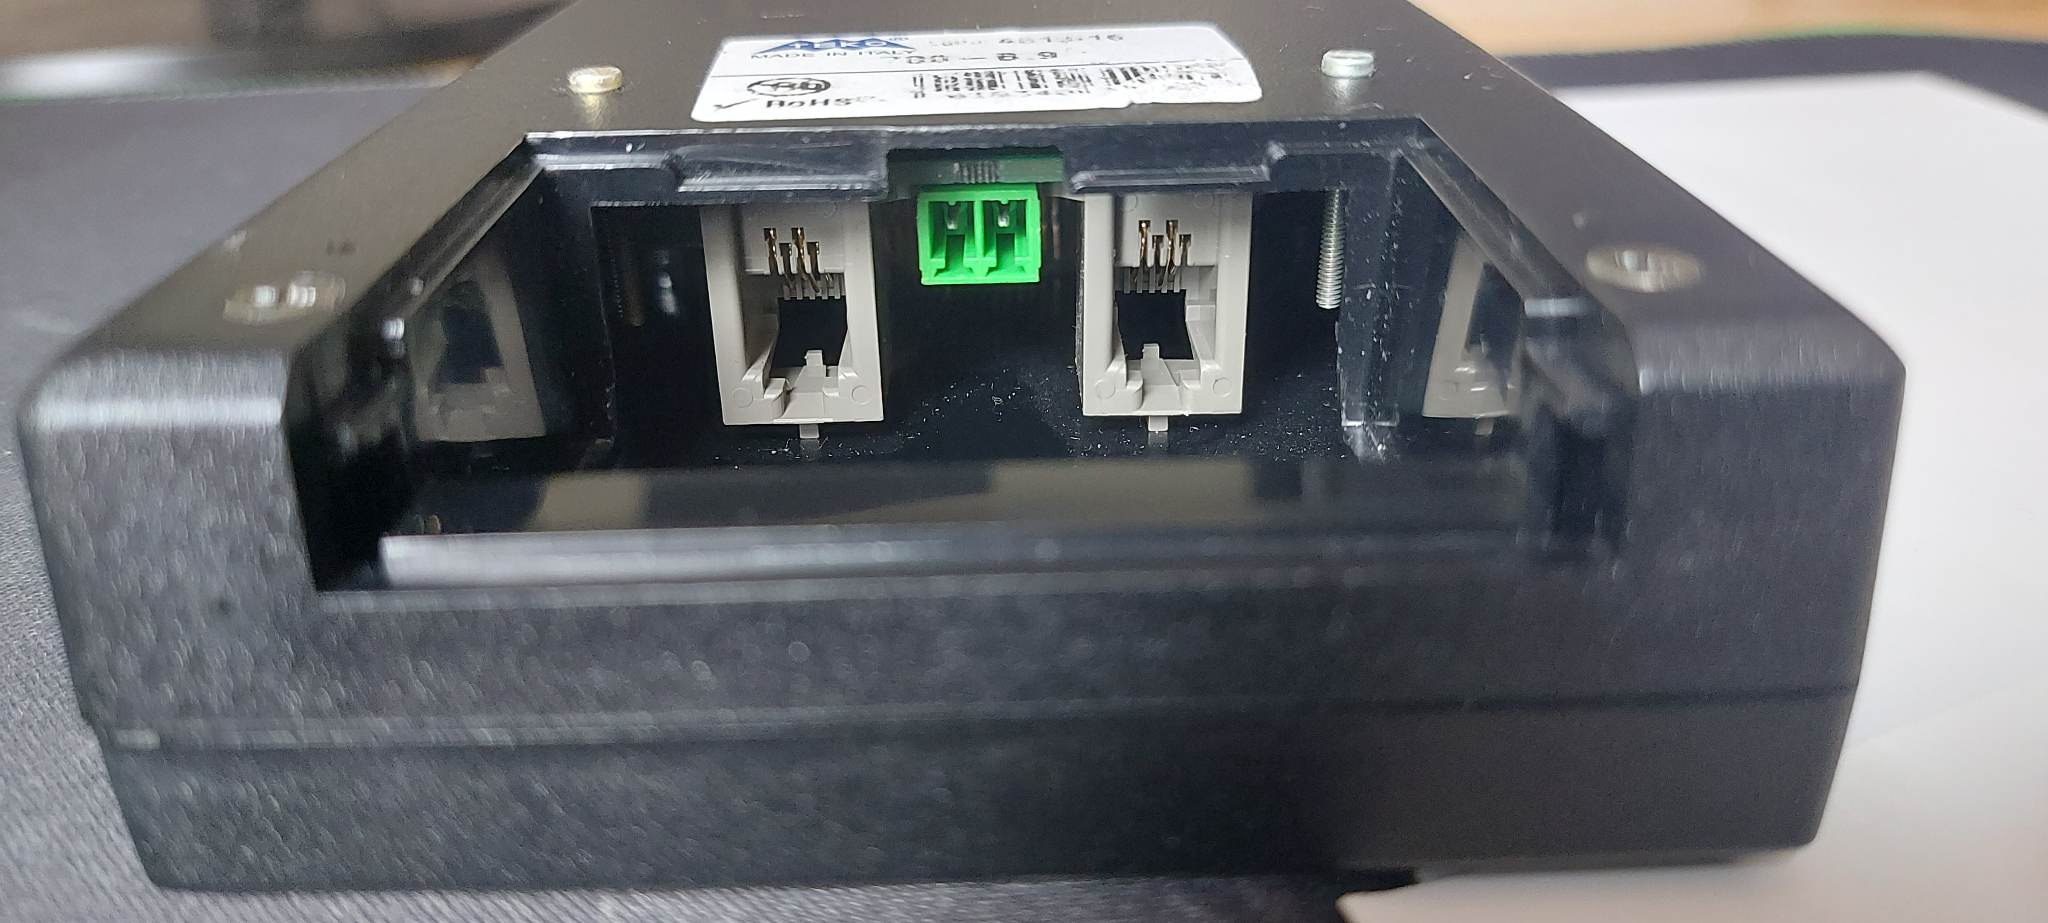
\includegraphics[page=1,width=0.5\textwidth]{táp,rj9}
		\caption[Eszközök aljzatai]{Eszközök aljzatai}
		\label{fig:csatlakozo}
	\end{figure}
	\newpage
	Az egyes egységeket láncszerűen kell egymás után kapcsolni, melyeket vagy individuálisan vagy kollektívan lehet kötni a vezérlő számítógéphez. 	\\
	Az eszköz tápellátásáért felelős aljzat a \ref{fig:tápcsatl} ábrán láthatjuk.
	\begin{figure}[H]	
		\centering
		\includegraphics[scale=0.5]{táp_csatl}
		\caption[Eszköz egyik áramellátásért felelős aljzata]{Eszköz egyik áramellátásért felelős aljzata}
		\label{fig:tápcsatl}
	\end{figure}
	
	\subsubsection{RJ-9-es csatlakozó}
	Az RJ-9-es csatlakozó kompakt, négyzetes kialakítású, és széles körben elterjedt a használata. A csatlakozó fej, felhasznált anyaga azért lehet érdekes, mivel áttetsző és akár ez esztétikailag is apellálóvá teheti az eszközt.
	A "pin"-jei különleges bevonatú anyagokkal rendelkezik amely megakadályozza az eszköz rozsdásodását. \cite{rj9Pros}
	Alapvetően az RJ9 vezetékes telefonokba használják, a telefon készülék és a kagyló közötti adatátvitel céljából.\cite{RJ9ok}
	Az eszköz RJ-9-es aljazata a \ref{fig:rj9csatl} ábrán található.
	\\
	\begin{figure}[H]	
		\centering
		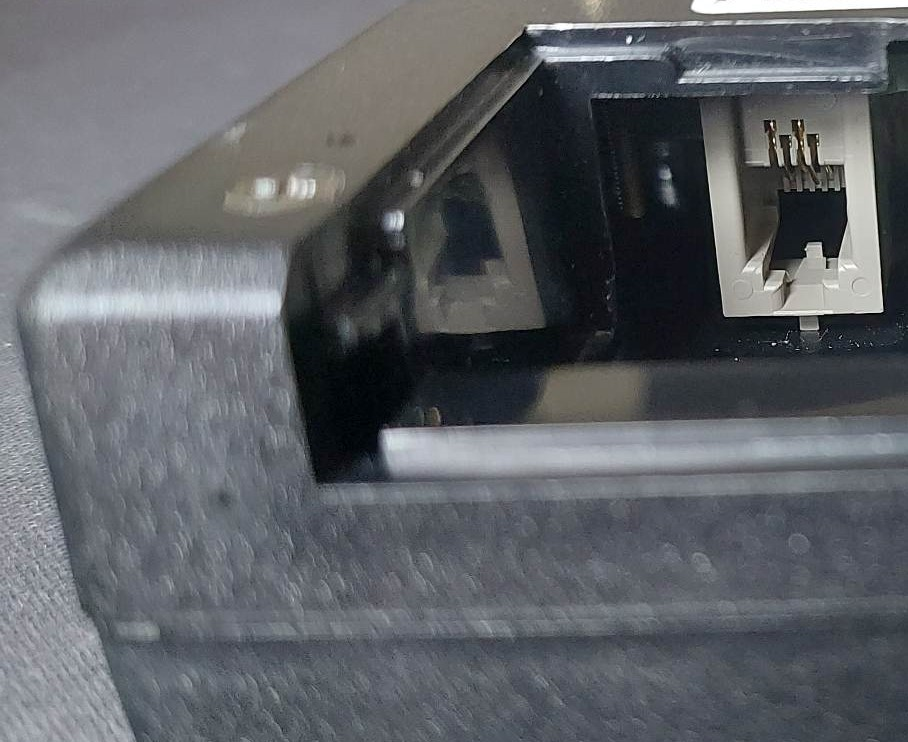
\includegraphics[page=1,width=0.4\textwidth]{rj9_csatl}
		\caption[Eszközök bemeneti portjai]{Eszköz RJ-9-es portja(bal oldali)}
		\label{fig:rj9csatl}
	\end{figure}
\newpage
	\subsubsection{USB-A és USB-B típus különbsége}
	A szabványos-A típusú USB csatlakozó, amely nagyrészt arra használatos hogy más USB bemenettel rendelkező eszközöket meghajtson. Ilyen például az USB-hub amely laptopoknál több USB portot szolgáltat.
	A szabványos-B típusú USB csatlakozó, amely főleg a perifériák vezérlése érdekében használatos. Ilyen perifériák például a nyomtatók, és a billentyűzetek. \cite{typeab}
	\\

	\begin{figure}[H]	
		\centering
		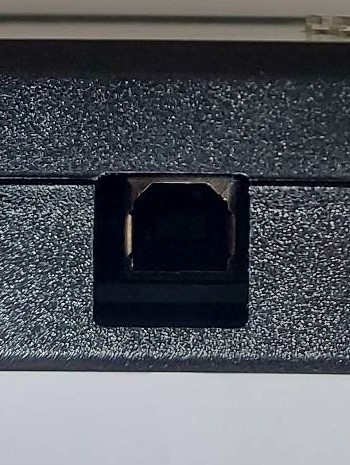
\includegraphics[scale=0.6]{lampa_usb2}
		\caption[Eszközök bemeneti portjai]{Eszköz USB Type-B aljzata}
		\label{fig:usb2_csatl}
	\end{figure}
	Az eszközhöz tartozó USB-B típusú aljzatról a \ref{fig:usb2_csatl} ábrán láthatunk egy fotót.
\newpage
	\subsection{Eszközök működtetéséhez szükséges kábelek}
	\label{eszkozokmukodtetese}
	Alapvetően önmagukban az eszközök nem funkcionálnak, szükségük van áramellátásra a működésükhöz. Erre kétféle megoldás létezik az eszközeinknél. \\
	Az egyik ilyen megoldás ha a USB-n keresztül kötjük össze az eszközünket valamilyen erőforrást generáló eszközzel, például egy hordozható Laptoppal. 
	\begin{figure}[H]	
		\centering
		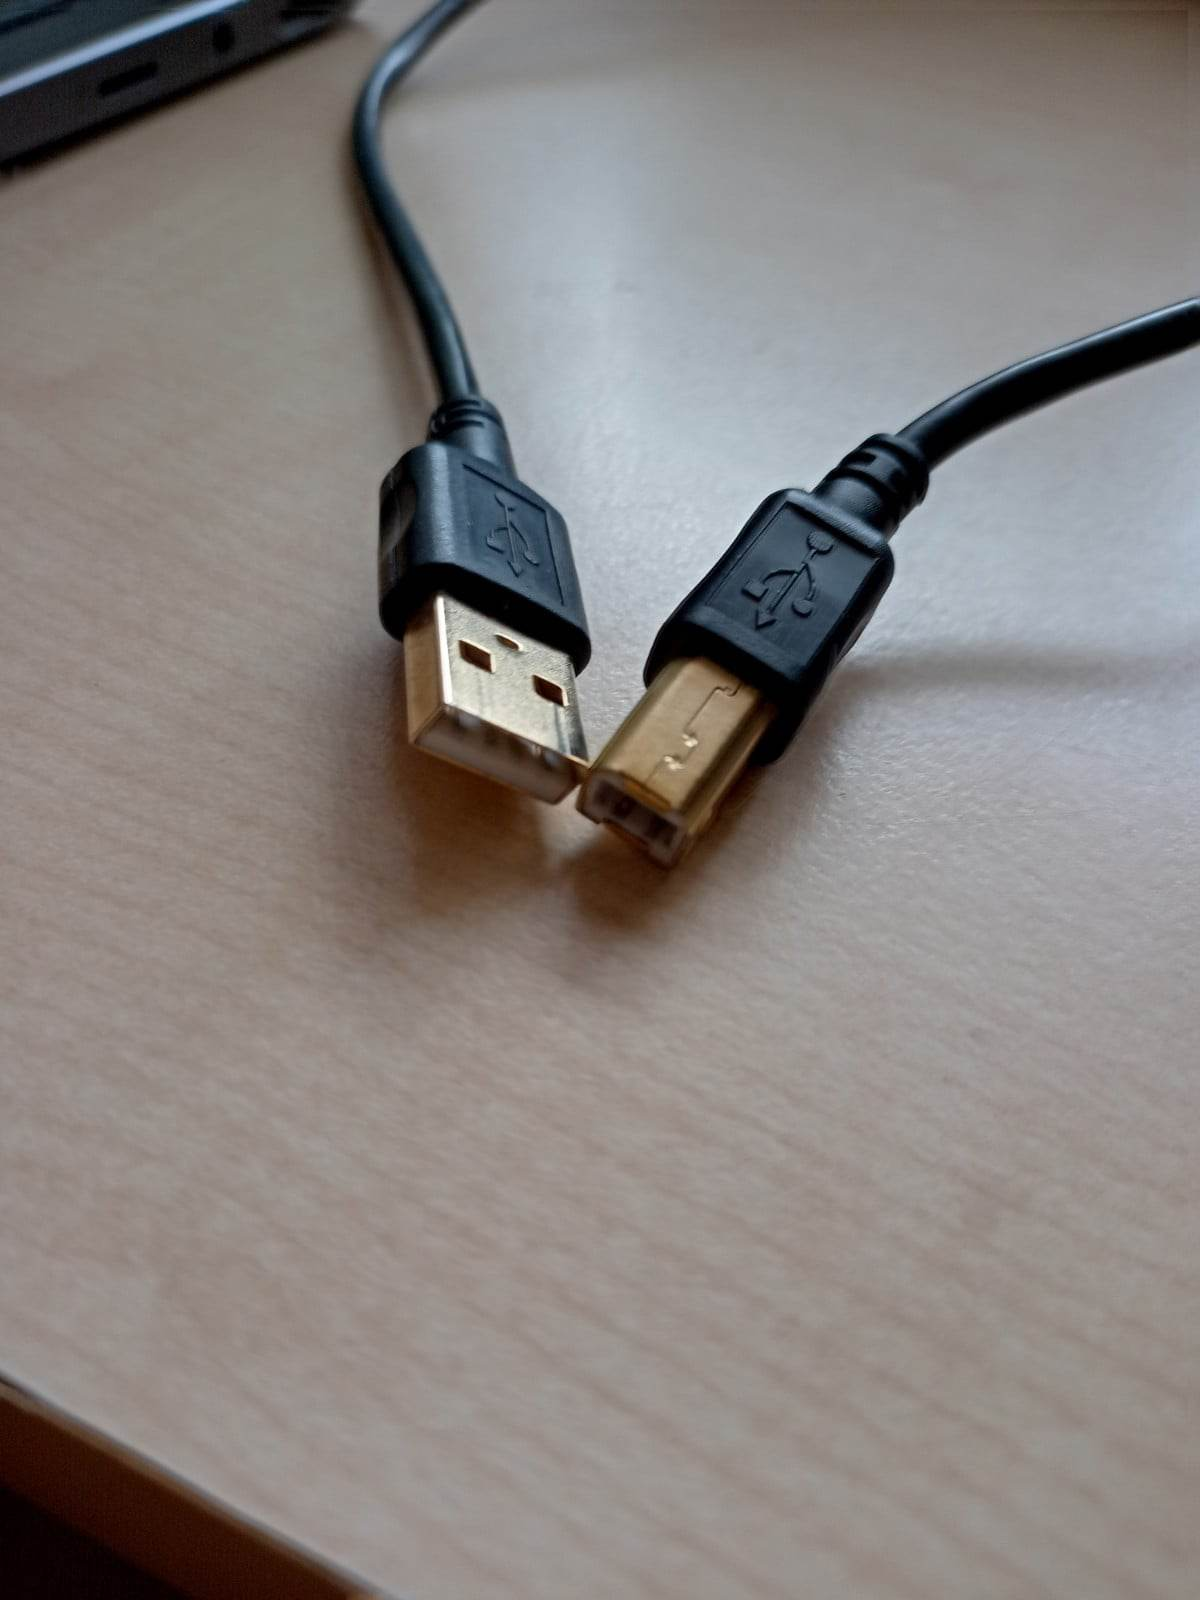
\includegraphics[page=1,width=0.4\textwidth]{USB}
		\caption[Nyomtató kábel]{Nyomtató kábel}
		\label{fig:USB_kabel}
	\end{figure}
	Ezen összekötéshez szükséges egy USB 2.0-ás nyomtatókábel, melynek az USB-B-s fele az eszköz USB-B-s aljzatába csatlakozik, és az USB-A-s fele pedig a tápot biztosító és programot futtató számítógépbe. 
	\ref{fig:USB_kabel}
	Ezen módszer segítségével képesek vagyunk, a megfelelő program segítségével egy eszközt működtetni individuálisan.
	\\
	A másik megoldás az, hogy felhasználjuk az eszközünkön lévő tápfeszültséget fogadó aljzatot, amelyet a \ref{fig:tápcsatl} ábrán láthatunk. Ezen aljzatba csatlakoztathatjuk a tápegységünket amely a \ref{fig:tapegyseg} ábrán található. Ez a tápegység egy SA124H-12G-s szériaszámmal rendelkező 24 Watt-os teljesítménnyel rendelkező egység, 
	amely képes egyénileg egy eszközt ellátni a megfelelő tápfeszültséggel. Az elektromos készülékek más és más feszültséggel és áramerősséggel működnek, ezért lehet jó a tápegységek használata. \cite{energom} 
	\begin{figure}[H]	
		\centering
		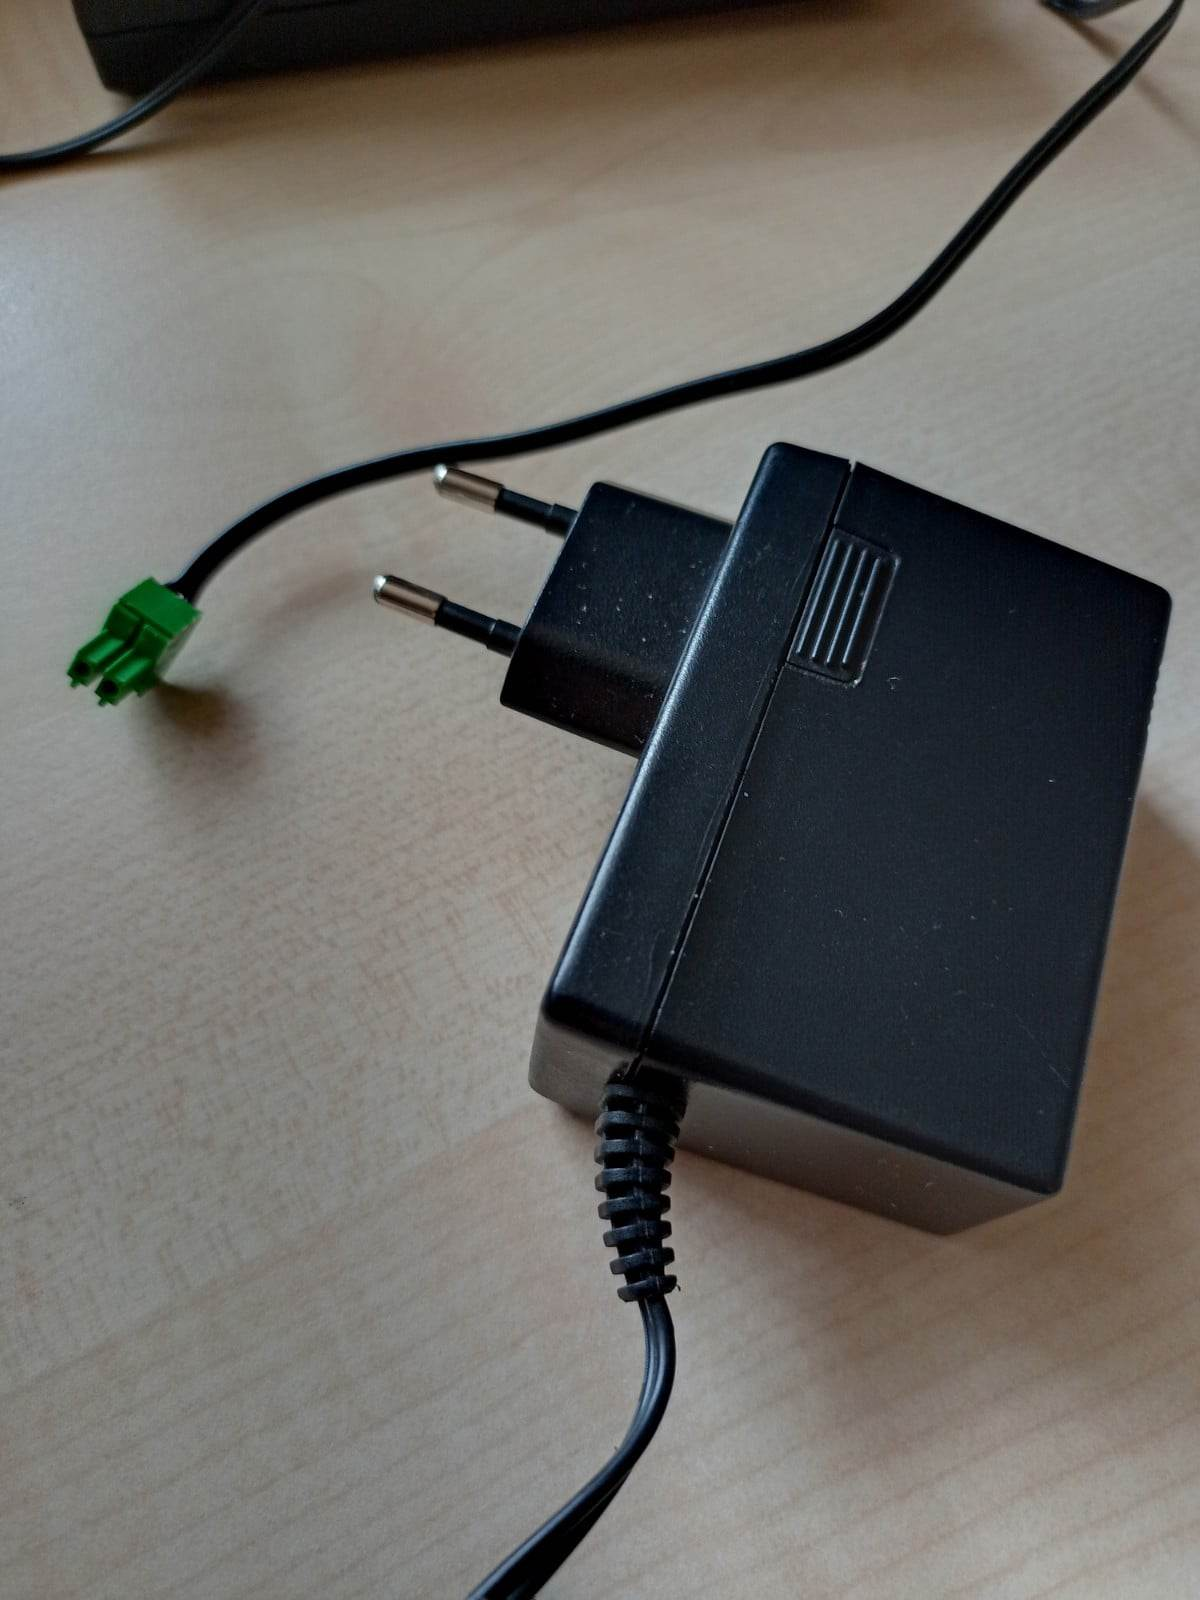
\includegraphics[page=1,width=0.4\textwidth]{táp_adapter}
		\caption[Tápegység]{Tápegység}
		\label{fig:tapegyseg}
	\end{figure}
	Fontos részlet az, hogy az eszköz beállítása ilyenkor még nem módosíthatóak, mivel nincs rákötve a programot futtató számítógépre. Ezt a problémát úgy tudjuk kiküszöbölni, hogyha felhasználjuk az RJ-9-es kábelünket a tápkábelünkkel együtt. Ez a kábel, képes arra, hogy az eszközeinket sorba kösse, és ezáltal működtethető lehessen egyszerre.
	Az RJ-9-es kábelről a \ref{fig:rj9_kabel} ábrán láthatunk képet. A kábel egyik végét az eszköz egyik RJ-9-es aljzatához kell csatlakoztatunk, majd ezt követően egy másik, a számítógéphez kötött eszközbe kell csatlakoztatnunk, ezzel elérve azt, hogy az eszköz sorba legyen kötve.
	\begin{figure}[H]	
		\centering
		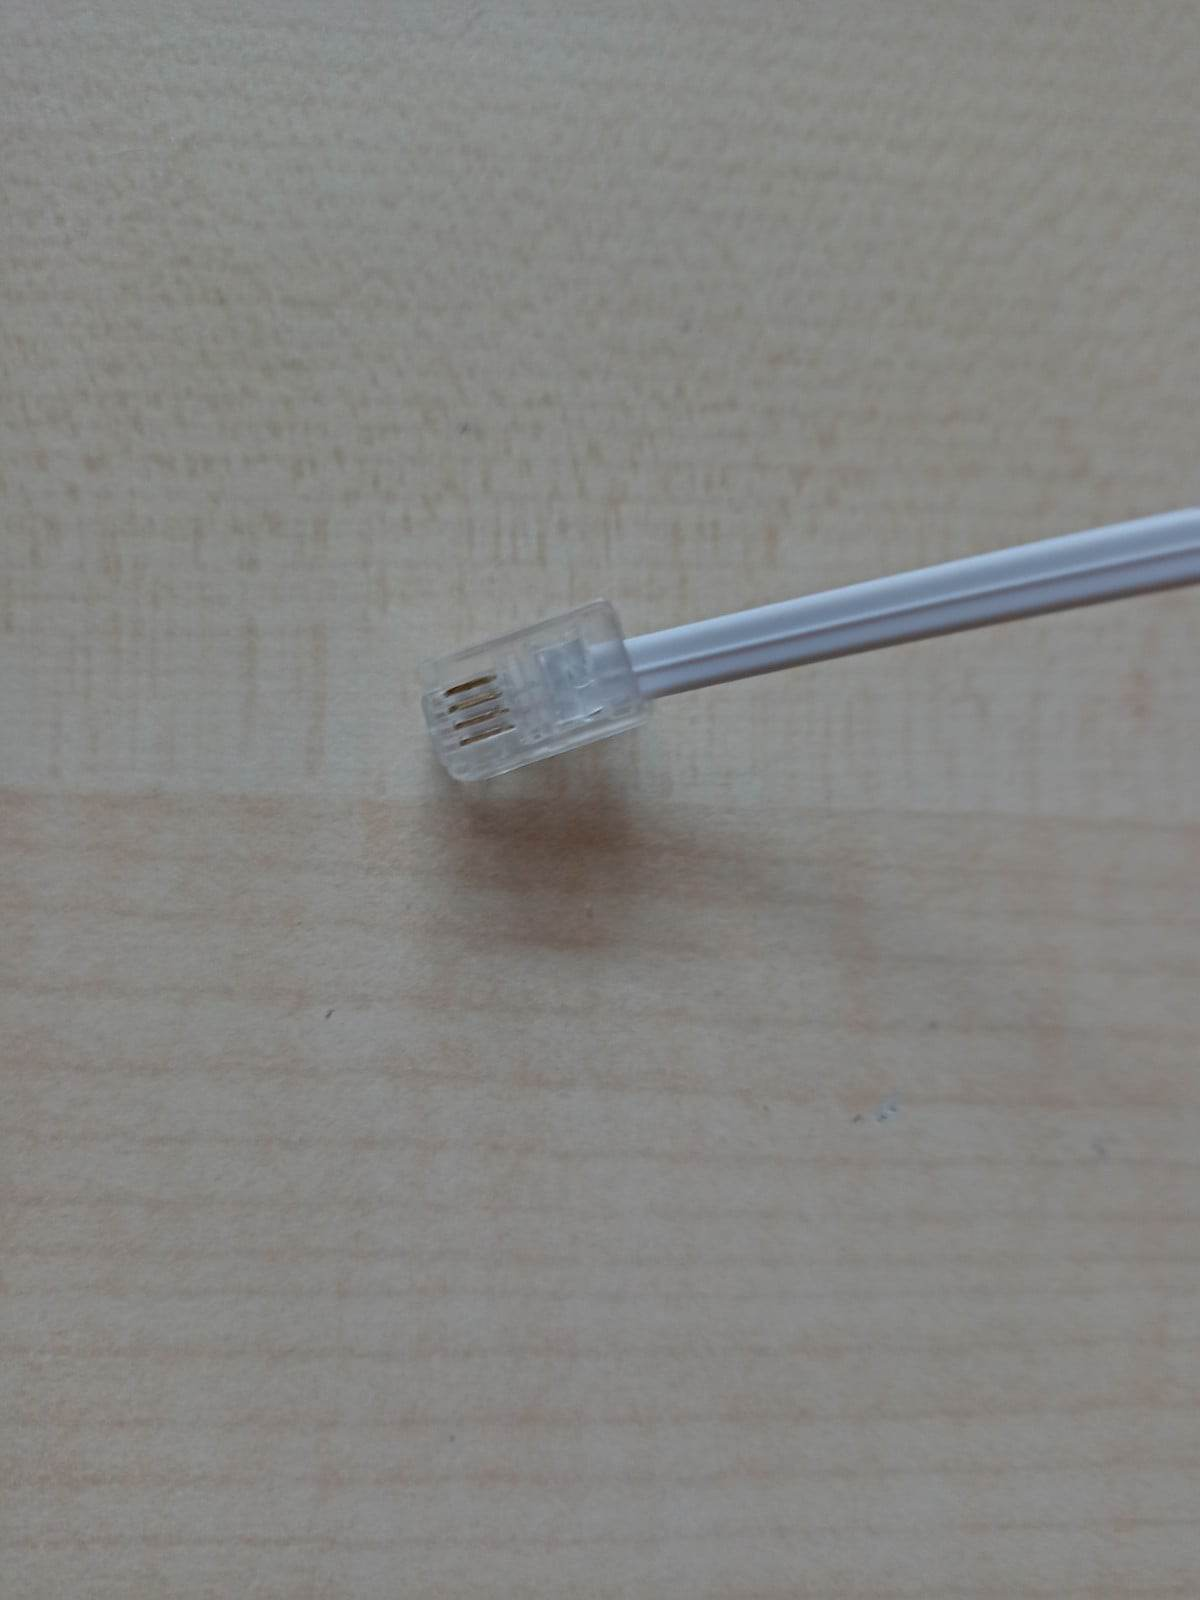
\includegraphics[page=1,width=0.4\textwidth]{rj9_kabel}
		\caption[RJ-9 típusú kábel]{RJ-9 típusú kábel}
		\label{fig:rj9_kabel}
	\end{figure}
\newpage

	\section{Felület tervezésének alapjai}
	A jelenlegi fejezetben magáról a lefejlesztett kódról és a nagyobb felhasználói élmény eléréséhez szükséges dizájn elemek bemutatásáról szeretnék beszélni. Továbbá, ezen felület kialakításához szükséges háttértudásokat szeretném bemutatni, amelyek nagyrészt elkerülhetetlenek egy ablakos alkalmazás fejlesztése során.
	\subsection{C\# fejlődése}
	A szakdolgozatom projektje C\# nyelven íródik amely a legjobban alkalmazkodik az ilyen felületek leimplementálásához. 
	
	A C\# nyelv alapvetően a Microsoft által kifejlesztett objektumorientált programozási nyelv.
	Ezentúl ez egy egyszerű, modern programozási nyelv amely egybeköti a C és a C++ nyelv erejét az új applikáció fejlesztésével egybekötve. \cite{hejlsberg2003c}
	\\ 
	Számos főbb újdonságokat implementáltak ebbe a nyelvbe, megemlítésre méltóak például a 2005-ös verzióban létrejövő Generikus és parciális típusok amelyek megkönnyítették a programozó munkáját, mivel általánosabb kódot tudtak írni ezek segítségével.
	Ezentúl, még hasonlóságokat is fedezhetünk fel például a Java nyelvben, amely egyezést mutat számos helyen.
	Mint például az osztályok deklarálása, metódusok illetve függvények létrehozása. Emellett a mezők szintaxisa is megegyező.
	\\
	A C\#-ban még sok más opciónk is van programok fejlesztésére, ilyen például a Konzolos Applikáció(Console Application), a Windows Forms Application, illetve a WPF(Windows Presentation Foundation). Ezen utóbbi kettő applikáció segítségével ablakos illetve asztali alkalmazásokat készíthetünk. \cite{almeida2018visual}
	\\
	A korábbi fejezetekben már említést tettem azon kapcsán, hogy az alkalmazást a C\# programozási nyelvben írom. Ezenfelül, egy olyan asztali alkalmazást szerettem volna készíteni amely apelláló lehet a felhasználó számára. Továbbá, a megjelenéstől, és a küllemtől eltekintve fontosnak tartom azt is, hogy amennyire csak lehet egyszerű legyen az alkalmazás használata.
	\\
	Az elkészített szoftver, főleg Windows operációs rendszerrel rendelkező eszközre készül, habár természetesen a .NET környezet támogatja a Linux, MacOS, Android illetve az IOS platformokat is, de fejlesztés szempontjából a Windows operációs rendszer tűnik a legkényelmesebbnek és a legegyszerűbbnek.\cite{altexsoft} Ezért az alkalmazás csak Windows eszközön lett kipróbálva és futtatva.
	\\
	A projektem során azért választottam a Windows Forms Application-t mivel a különböző eszközök(gombok, címkék) amelyek az ezen alkalmazásban megtalálhatóak elősegítik a felhasználó számára a könnyed olvashatóságot és feltérképezés lehetőségét. Az alkalmazás hasonló módon elkészülhetett volna konzolos felületre is, de mivel ez a felhasználó és az esetlegesen laikus ügyfél számára is nehezen érthető, ezért az ablakos alkalmazás a támogatott.
	\\ 
	\subsection{Dynamic Link Library mint erőforrás}
	C\#-ban lehetőség van úgynevezett DLL-ek használatára is. A DLL(Dynamic Link Library) mint olyan az egy kisebb programok összessége, amelyeket nagyobb programok könnyűszerrel be tudnak importálni a saját projektjükbe. Ezen kisebb programokhoz vagy DLL fájlokhoz, hozzátartozik leírás is amelyek általában minden egyes függvényeknél, illetve metódusoknál megjegyezhető. Ennek oka, hogy az a fejlesztő aki használja a DLL-t
	nagyobb belátást kapjon arról hogy az adott metódus, miként és hogyan működik.\cite{benlutkevich}
	\\
	A projekthez a DLL-t, Nagy-Tóth Bence hallgatótársam szolgáltatja amelyben számos metódus meg lett írva, ezeket felhasználva a fő applikáció működésre bírható.
	\\
	Ezentúl, a működtetett eszközökkel való kommunikáció alapját Delphi programozási nyelvből indulva C\# nyelvre lett implementálva amely a DLL és a felület alapját képezte. A programkódjáról egy részlet a \ref{fig:dllbence} ábrán találjuk. 
	\begin{figure}[H]	
		\centering
		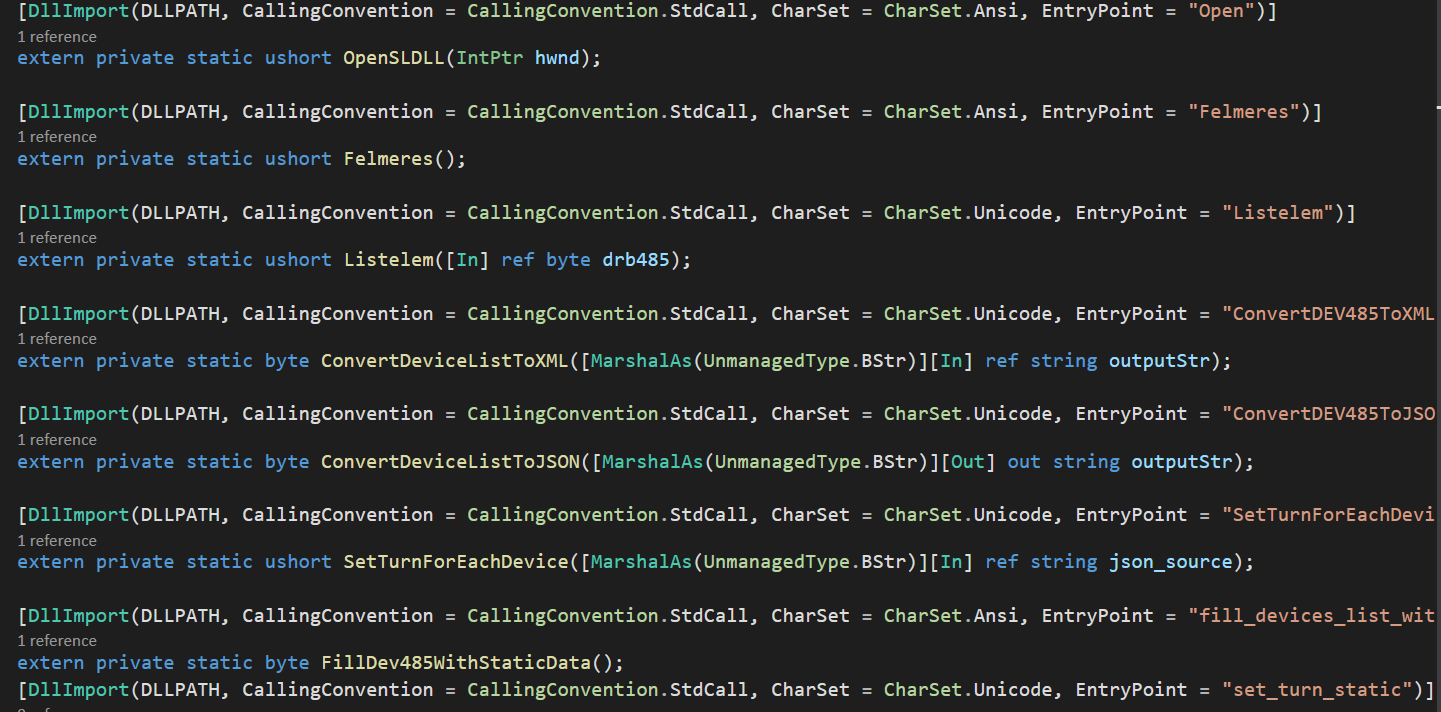
\includegraphics[scale=0.3]{DLL_bence}
		\caption[C\# DLL kódrészlete]{C\# DLL kódrészlete(főbb metódusok)}
		\label{fig:dllbence}
	\end{figure}
	
	Miután elindítjuk a szoftvert azután USB port-on keresztül lehet kommunikálni az adott eszközökkel, mint ahogyan arról említést is tettem a \ref{eszkozokmukodtetese} fejezetben is.
	Maga a felület, nem teljes képernyős módon lett lefejlesztve, hanem egy statikus érték alapján nézhetjük az alkalmazást.
	Ennek oka, hogy az alkalmazás elsősorban egy okos telefon képernyőjénél nagyobb képernyőkre lett tervezve, ezért nem találtam lényegesnek a kisebb eszközökhöz való adaptálását.
	Kutatásom során találkoztam egy olyan dizájn formával ami kifejezetten szépnek és modernnek bizonyult számomra.\cite{modernUI} 
	Ezt a megjelenést egy nyílt forráskódú kód és publikus videó alapján készítettem, amely segítségemre volt a dizájn elképzelésében.\cite{rjcode}
	Maga a felület több részből épül fel amelyet a következő alfejezetekben taglalok.
	\\
	\subsection{Windows ablakos felület tervezés}
	A Windows Forms-on belül számtalan lehetőségünk van a felületünk  megtervezésére. Lehetőségünk van nézetet választani az egyik amely az alap tervezői nézet, és emellett természetesen az alkalmazásunkat kód formájában is megírhatjuk. Számomra a kettő nézet ugyanolyan releváns a projekt szempontjából, mivel a tervezői nézetben, ténylegesen átláthatjuk, hogy a felhasználó mit fog látni, mint végtermék.
	
	Amikor a kódnézőben tartózkodunk, akkor természetesen eltudjuk érni a ugyanazokat az eszközöket amelyeket a Designer nézetben is.
	Ebben a szekcióban, különböző működési elveket és formai adatokat írhatunk le amelyek meghatároznak különböző objektumokat a form-on belül. \cite{appSysWinform}
	\subsubsection{Designer nézet}
	A nézet választás fontos, és egyben jár a programozás részével is, mivel amikor akár egy gombbot akár egy címkét helyezünk be a képernyőbe akkor is a háttérben történnek változások a kódban is.
	
	A tervezői nézetben egy üres formra építhetünk különböző objektumokat.
	Ez egyszerűbb lehet sok fejlesztő számára mivel, az eszközöket amiket eltudunk helyezni a formunkon mind megtalálható a "Toolbox" nevezetű oldalsávon belül.
	\\
	Itt találunk számos eszközt amelyek bármelyikét használhatjuk a formunkon. Ilyenek például a buttonok vagyis a gombok, vagy a Labelek vagyis a címkék és továbbá elérhetőek még maguk a panelek vagy alpanelek is. 
	\\
	Amikor elhelyeztük a kívánt kelléket a formon akkor lehetőségünk van többféle beállításra az adott tárgynál. ezek közé tartozik az az opció amikor egy adott objektumnak a hátterét, címét és még sok más tulajdonságát lehet változtatni a kiválasztott eszköznek. Ezentúl még adott eszköznek lehetnek eseményei is amelyek egy adott impulzus alapján (például: bal klikk lenyomása egy gombbon) kiváltanak egy másik akár látható akár nem látható reakciót a programon belül. Ezekről bővebben az Eszközök című [\ref{EszkozLista}] alfejezetben írok.
	
	\subsubsection{Alap kód nézet}
	
	A Designer vagy tervezői nézet mellett a programozóknak alkotott nézet is megtalálható a WinForm applikáción belül. Ez a nézet az alap kódolói nézet, amely ugyanolyan fontossággal bír mint a Designer nézet.
	\\
	Amíg a Designer nézetben főleg azon volt a hangsúly hogy a Form-nak vagyis a képernyőnek a nézetét kialakítsuk, megformázzuk. Ezzel ellentétben a kódolói nézetben nem feltétlen látjuk azonnal a kívánt produktumot, mivel ez csak indításkor jelenik meg számunkra, amikor "\textit{lebuildeljük}" a programunkat. Ezt az indítást akár a gyorsbillenytű (\textbf{F5}) segítségével tehetjük meg, vagy a zöld nyílra kattintva a lap tetején.
	\\
	A kódolói nézetben a programozónak lehetősége van minden C\# specifikus elem kihasználására. Alapvetően a minden egyes Gyermek Form örökli a Szülő Form minden public, illetve protected metódusát és mezőjét. 
	\\
	\subsubsection{Initialize Component metódus}
	A Formoknál mindig van egy inicializáló konstruktor, amely meghívja a(z) \textit{InitializeComponent()} nevű metódust amely az automatikusan megírt kód alapján előkészíti a form képernyőt a különböző objektumok fogadására. Egyúttal, ez a metódus alapozza meg a gombok, címkék, esemény kezelők és még több ilyesfajta objektumoknak a későbbi beillesztését és használatát.
\\
Ezen kívül, az említett metódus megkeresi a betöltődő Képernyő(Window) és a Felhasználó Vezérlő(UserControl) XAML-jéhez tartozó URI-t.
\\
Majd átadja azt a System.Windows.Application.LoadComponent() nevezetű statikus metódusnak.
Ezt követően, a LoadComponent() nevezetű metódus betölti az átadott URI-n található XAML-fájlt, és átalakítja azt az XAML-fájl gyökéreleme által megadott objektum példányává.
\\
\subsubsection{XAML nyelv}
Az \textbf{XAML}(angolul: Extensible Application Markup Language) mint olyan alapvetően egy deklaratív nyelv, amely XML alapján képződött.
Emellett az XAML főleg az olyan típusú eszközök programozásánál használatos amikor felhasználói felületet kell készíteni és programozni. Ilyenek például a Windows Presentation Foundation (WPF) amely sok hasonlósággal rendelkezik a Windows Forms-hoz is.
\\
\subsubsection{Uniform Resource Identifier, URI}
Az \textbf{U} egységesség(Uniform) számos előnnyel jár. Lehetővé teszi a különböző típusú
erőforrás-azonosítók ugyanabban a kontextusban használhatók, még akkor is, ha az erőforrások eléréséhez használt mechanizmusok különbözhetnek.
\\
Az \textbf{R} olyan a specifikáció amely, nem korlátozza annak körét, hogy mi lehet az erőforrás. Az "erőforrás" kifejezés inkább általános értelemben használatos mindenre, ami URI-val azonosítható. Ilyenek lehetnek az elektronikus anyagok, képek, egy adott információról kapott forrás valamilyen következetes céllal.
\\
Az \textbf{I} az azonosító megtestesíti azokat az információkat, amelyek ahhoz szükségesek, hogy az azonosított dolgot megkülönböztessék az olyan azonosított dolgoktól amelyek az információk hatáskörébe tartoznak.\cite{uri}
Az "azonosító" és "azonosítás" arra a célra utal, hogy megkülönböztessenek egy erőforrást az összes többi erőforrástól, attól függetlenül, hogy az milyen célra lett kihelyezve.  
\\
Mind az URI és az XAML is fontos szerepet tölt be, a C\# nyelvbe épített alapmetódusaiban.
	\subsection{Eszköztár}
	\label{EszkozLista}
	Az eszközök listáját használhatjuk a Designer nézetben. Ezzel a módszerrel, könnyedén tudjuk mozgatni az adott eszközöket. Emellett, az Eszköztár ablakban a vezérlőelemek jelennek meg.Az eszköztár megnyitásához a menüsorból a Nézet > Eszköztár parancsot kell megkeresni, vagy a \textbf{Ctrl+Alt+X} billentyűzetkombinációt kell megnyomni. Ilyenek például a gomb, címke, panel. Az eszköztár a tervezői nézetekkel együtt jelenik meg általában. 
	\\
	Az eszköztárban lehetőségünk nyílik szűrni is különféle eszközökre, ezt megtalálhatjuk a \textit{Search Toolbox} nevezetű kereső mezőben.
	\subsubsection{Gombok}
	\label{Gombok}
	A gombok általánosságban olyan fontos elemei a felületnek és a Formnak is amelyeken keresztül nem csak a programozó kommunikálhat a felhasználó felé, de a felhasználó is kommunikálhat a program illetve a programozó felé. 
	\\
	Ezentúl még a gombok hasznosnak bizonyulnak sok különböző helyzetben is mivel a gomboknak és más objektumoknak is, léteznek úgynevezett eseményei. Ezen eseményeket (Angolul: "Event") a felhasználó ki tudja váltani különböző cselekedetekkel. Ilyen esemény lehet példaként az amikor a felhasználó a bal egér gombbal kattint a gomb felületére, ezzel kiváltva egy eseményt ami bekövetkezik ezen okból kifolyólag.
	\\
	Tervezői nézetből egy gomb esemény kialakítása többféle módon történhet. Amikor kihelyezzük a használni kívánt gombot akkor lehetőségünk van, vagy a jobb alsó sarokban megjelenő "\textit{Properties}" nevezetű ablakon belül navigálni vagy egyszerű módon csak kétszer kattintunk a létrehozott gombra, ezzel a programunk legenerál számunkra egy "xyz\_Click()" metódust.
	Az elsőnek említett módban, a "\textit{Properties}" nevezetű ablakon belül, az apró villám ikonra kell kattintanunk, amely az adott objektumhoz tartozó események listáját tárja szemünk elé. Ez megkönnyítheti a kereséseinket, hogy éppen az adott objektumra milyen események lehetségesek. További információt majd a \ref{esemenyformban} fejezetben fejtenék ki.
	\subsubsection{Címkék}
	\label{Címkék}
	A címkék általánosságban megtalálhatóak minden programban felületén. Ilyenek például az üdvözlő üzenetek, címek, szöveges magyarázatok.
	%ide akár lehetne ezekről ilyen képeket is betenni a címkékről
	A címkék alapvetően nem arra szolgálnak, hogy a felhasználó tudjon kommunikálni a programozóval/programmal, hanem arra, hogy a fejlesztő tudja továbbítani a programozó által írt szöveges üzeneteket a felhasználó számára. Hasznos lehet olyankor amikor a felhasználóval tudatni akarunk olyan információkat amelyek a  program működéséhez releváns volna. Ennek egy példája amikor egy adott gombnak a funkcióit szeretnénk leírni, ilyenkor a címke arra szolgál, hogy feliratozzuk az adott funkciókat a programunkon belül.
	\\
	  Természetesen mind a kétféle nézetben(designer/kód) elérhető számunkra a címkék használata, de meg kell fontolnunk, hogy kód nézetben alapvetően nem látjuk azonnal azt amit a felhasználó is látni fog, ezért talán nehézségekbe ütközhetünk ilyenkor ha manuális szeretnénk kód formájában megadni a címke paramétereit, beállításait. Amennyiben designer nézetben helyezzük el a címkénket könnyebben és rugalmasabban tudunk a programunkkal dolgozni, de sajnos ennek is megvannak a hátrányai, ha a program futási idejében szeretnénk változtatni akkor használnunk kell a kód nézetet is amellyel kiegészítve megtudjuk oldani ezeket a felmerülő problémákat is. Ebből kifolyólag hasznos lehet a designer nézet és a kód nézet együttes dinamikus használata.
	  \\
	  Mivel a címkék is szövegek/stringek ezért egy adott címkének el lehet érni a szöveg formátumát sok más beállításával együtt. Ilyenkor ha stringet szeretnénk esetlegesen konkatenálni, abban az esetben az adott label-nek a \textit{Text} nevezetű property-jét kell lekérdeznünk. Majd ezt követően használhatjuk a címkénk szöveg adására, illetve kiegészítésére.
	\\
	Későbbiek során természetesen ez a funkció is szerves részét alakítja az elkészült programnak.
	\subsubsection{Panel}
	\label{Panel}
	A formnak mint olyannak léteznek paneljei. Ezen panelek hasznosnak bizonyulnak sok szempontból. Legfőképpen a háttér díszítéséhez, objektumok összegzésére lehet használatos. Jelen alkalmazásban is két fő részében használom a projektnek. 
	Oldalsávhoz használtam fel a panelt, illetve a fejléchez. 
	\\
	Ahhoz, hogy a panel fejléc illetve oldalsávként funkcionáljunk néhány beállítást kellett elvégezni a panelen. A fejléc kialakítását az úgynevezett \textbf{Dock} nevezetű beállítással lehet konfigurálni. 
	 \\
	 A Dock abban segít hogy egy adott objektumot a képernyő egy adott részére helyezze, feltűzze. A megoldás segít abban, hogy reszponzív maradjon a felület, és egy szép kialakítást biztosít számunkra a megjelenítést illetően.
	 \\
	 Az oldalsávot is hasonlóképpen lehet megoldani, mindösszesen a Dock beállítást kell bal vagy éppen jobb oldalira konfigurálni, és ezzel a képernyő oldalához illeszti a panelt.
	\subsection{Delegatek}
	\label{Delegateek}
	A delegatek a C\# nyelven belül, mindig egy hivatkozás. Egy olyan hivatkozás amely mutat egy metódusra. Amennyiben egy delegatet hívunk akkor a hivatkozott metódus lesz meghívva. A delegateknek megvan minden szükséges információjuk ahhoz, hogy hívják egy adott egyedi névvel és visszatérési típussal ellátott metódust vagy metódusokat.
	\\
	A delegateket átadhatjuk egy másik metódusnak is ezzel áthelyezve a metódusnak a felelősséget a híváshoz, vagy éppenséggel egy struktúrában vagy osztályban is tárolhatjuk a delegatejeinket. A delegateket akkor használjuk, amikor nem tudjuk, hogy melyik metódust fogjuk meghívni tervezés közben, hanem csak futás közben derül ki ez.
	\\
	A delegatek deklarálásához szükséges a \textbf{delegate} kulcsszó amelyet követően meg kell adni a visszatérési értéket és a delegate nevét és paraméterét.
	\\ 
	Ezt követően meg kell írnunk a hivatkozni kívánt metódust, majd ezek után a delegatet és a metódust összekötjük úgy, hogy a delegatet lepéldányosítjuk és a new kulcsszót és a delegate nevét követően paraméterben megadjuk a kívánt metódust. 
	\\
	A delegatekre a későbbiek során csak az eventek során lesz szükségünk, mivel az eventek alapját képzik a delegatek felhasználása.
	\subsection{Események}
	\label{Eventek}
	Az események vagy eventek \cite{evinC} a C\# nyelven belül, olyan mechanizmusok, amelyeket az osztályok használnak értesítések vagy üzenetek küldésére más osztályoknak. Az események számos alkalmazás létfontosságú részét képezik, és tökéletes módja annak, hogy rugalmas és bővíthető alkalmazásokat hozzunk létre.
	Az elkészített alkalmazás is számos helyen alkalmaz, eventeket amelyek általában gombok lenyomásakor történnek meg.
	\\
	\subsubsection{Esemény készítése}
	Ahhoz hogy egy eseményt megalakítsunk szükség van egy kiadóra, aki az eseményt létrehozza, majd az esemény fogadásához és kezeléséhez elengedhetetlen egy fogadó is aki feliratkozik az esemény fogadására.
	
	\subsubsection{Esemény a gyakorlatban}
	Az event emellett általában a megfigyelő tervezési mintával kapcsolatban használják. Amikor ugyanis egy ilyen esemény bekövetkezik a feliratkozott figyelők csoportja meg lesz szólítva és ezzel kapnak információt a bekövetkezett eseményről. Azok az objektumok amelyek "érdekeltek" abban, hogy fogadjanak értesítéseket az eseményről, azok regisztrálnak egy delegate példányra az eseményhez.
	Egy esemény mindig a vele együtt elérhető delegattel van definiálva. 
	Az eseményt mindig egy delegattel kell együtt használni.
	\\
	Egy esemény értéke \textbf{null}, ha nincs regisztrált/feliratkoztatott figyelője/hallgatója.
	\subsubsection{Esemény működtetése a formban}
	\label{esemenyformban}
	Egy Formban általában alap eszközökre vagy objektumokra hozhatunk létre eseményeket, ilyenek például egy gombra való kattintás, vagy esetlegesen egy textbox nevezetű elem amelybe éppen megváltoztattuk a szöveg tartalmát.
	Számos lehetőségünk van az ilyen eszközökből kiváltani eseményeket.
	Az események létrehozásáról már a \ref{Gombok} számú fejezetben említést tettem.
	Miután elkészítettük ezeket az eseményeket akár a "Properties" ablakban akár másféle módon utána a létrehozott metódusunk egy \textbf{private} láthatósági móddal rendelkező metódus lesz, amelynek visszatérési értéke \textbf{void} vagyis visszatérési értékkel nem rendelkezik. 
	\\
	Ezentúl, paramétereiben kettő objektumot kap meg a metódus, egyrészt egy \textbf{object sender} amely az eseményt kiváltó vezérlőre/objektumra való hivatkozást tartalmazza. Tegyük fel, hogy egy képernyőn több gomb van. Ezek a gombok tartalmazhatnak egy címkét, amely leírja, hogy mit kell tennie a gombra kattintva. Ezáltal az összes \textbf{"Click"} eseményt lehetséges lekezelni ugyanazzal a handlerrel.
	Emellett egy \textbf{EventArgs e} objektumot amely az eseményadatokat tartalmazó osztályok alaposztályát képviseli, és egy olyan értéket biztosít, amelyet az eseményadatokat nem tartalmazó eseményekhez kell használni. 
	\cite{eventobjargs}
	
	\section{A projekt Formjai}
	Alapvetően a projekt több képernyőből áll, mindegyik az alkalmazásban megtalálható menüponthoz egy külön form tartozik, amely a kód szeparálhatóságát tette lehetővé.
	A képernyőket próbáltam megoldani az előző fejezetekben említett módon, hogy szép és modern lehessen. Mind ehhez fontos volt azt elérnem minden egyes képernyőnél, hogy átláthatóak lehessenek a képernyőn lévő funkciók.
	\\



\begin{comment}
	\subsection{SzinTema osztály}
	A \textbf{SzinTema} nevezetű osztály egy külön készített nem beépített osztály, amely a színváltozásokat és az alap színkódokat tárolja el.
	A színkódokat egy Listában tároljuk el amelyből majd a későbbiekben a Form Main Menu Form választja ki a megfelelő színeket. Ehhez a listához van egy \textbf{getColorList()} metódusa is amely a listának az elérésére szolgál. 
	\\
	A másik metódus az a \textbf{ChangeColorBrightness()} metódus amely paraméterében vár egy \textbf{Color} példányt illetve egy korrekció faktort amely a színek korrigálását fogja végezni, ezzel elérve a várt színárnyalatokat. Amennyiben túl sötét lenne a szín vagyis a korrekció faktor nagyobb lenne mint 0 akkor a színét kivilágosítjuk, ellenkező esetben a korrekciófaktort növeljük 1-el és megszorozzuk őket a piros, zöld, illetve a kék színértékekkel. Ezt követően visszatérési értékként visszaadjuk a megkapott színt mint visszatérési érték.
\end{comment} 
	\subsection{Form Main Menu}
	\label{FormMainmenu}
	Az első Form, a főmenü, vagyis amikor a felhasználó megnyitja az alkalmazást akkor ez az első képernyő ami számára megjelenik. 
	Ezen képernyőn egy üdvözlő üzenetet kap, majd az észlelt eszközök darabszámát is látni fogja, amely ugyanúgy megjelenik a képernyőn.
	Az üdvözlő üzenet, a fejlécen, a Form tetején jelenítjük meg amely egy Panel segítségével kapott színes hátteret.
	\\
	Eleinte a képernyő fejlesztése során felmerültek különböző problémák.
	Ebbe beletartozik az, hogy egy képernyőn kicsit zsúfoltan voltak elhelyezve a gombok, címkék.
	\begin{figure}[H]	
		\centering
		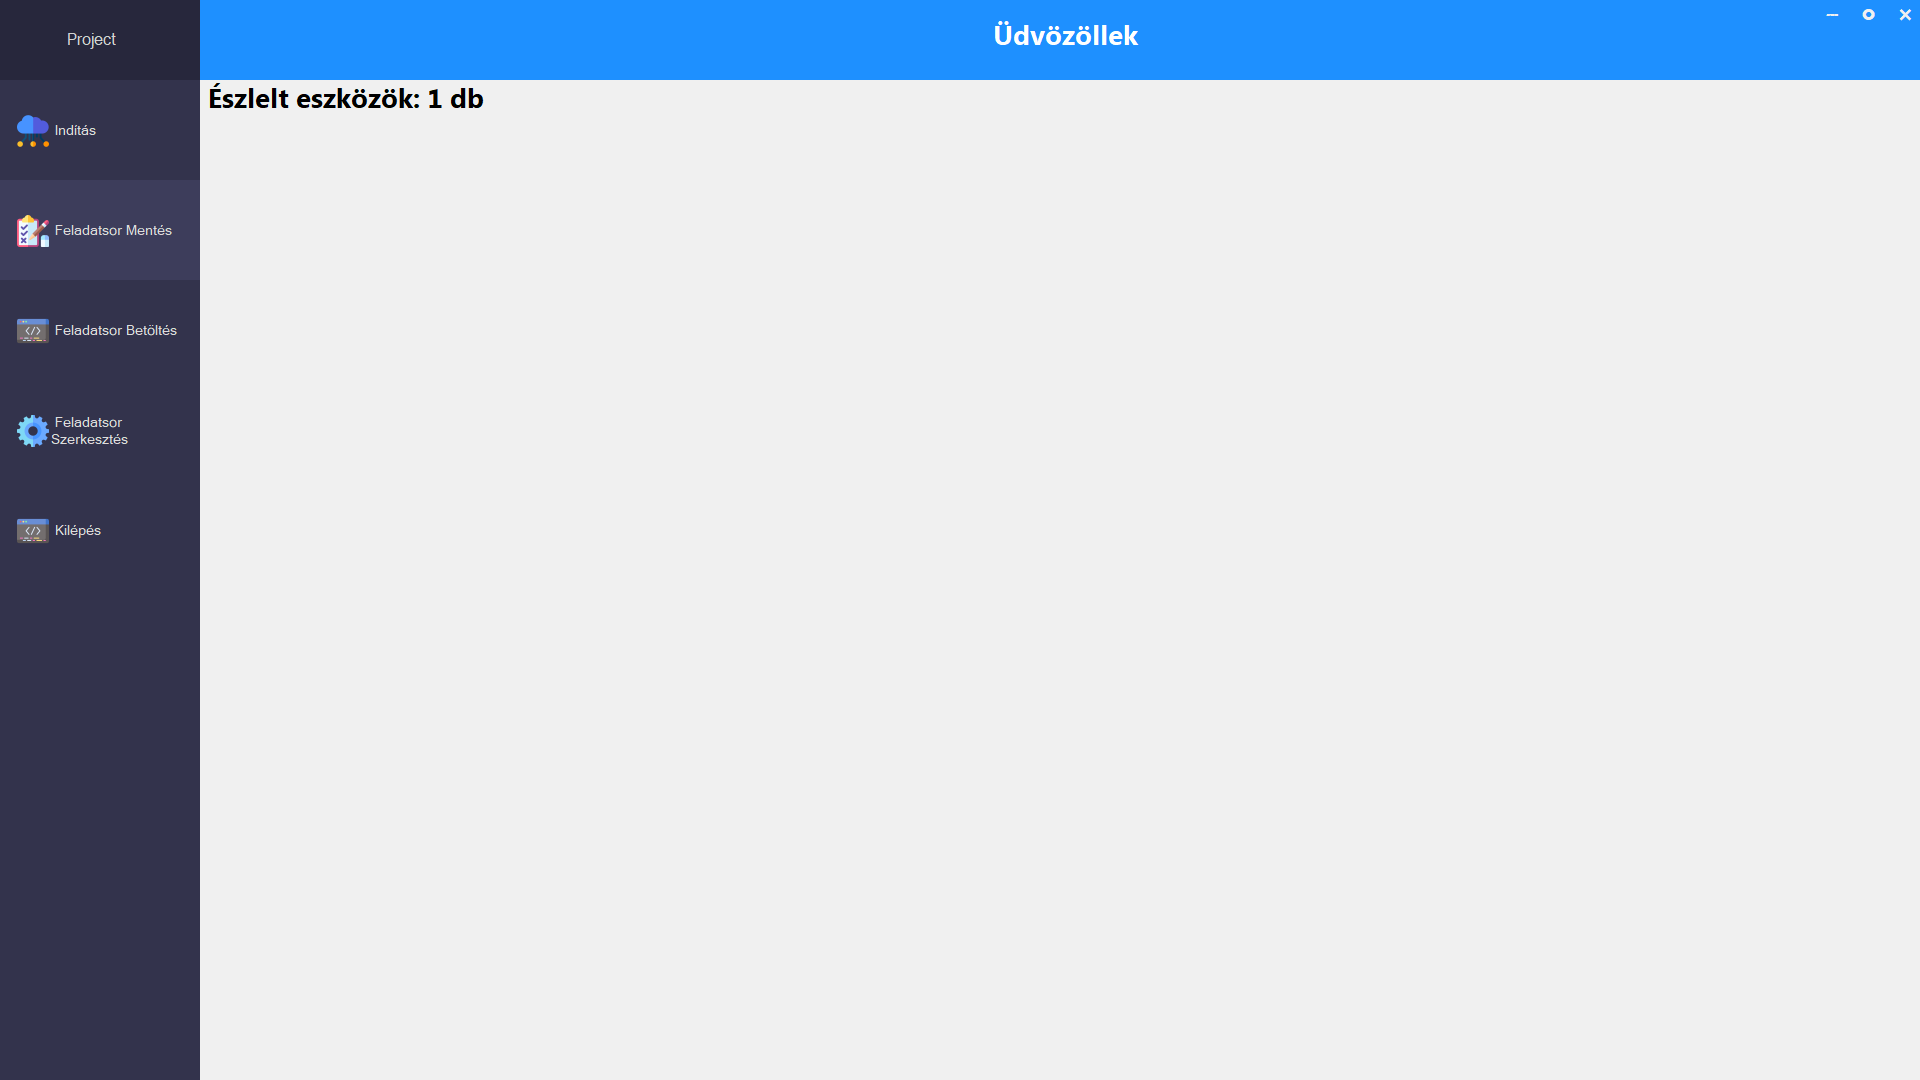
\includegraphics[scale=0.2]{prototipus_main_menu}
		\caption[Kezdő képernyő kezdeti fázisban]{Kezdő képernyő kezdeti fázisban}
		\label{fig:main_menu_start}
	\end{figure}
	A \ref{fig:main_menu_start} ábrán is látható hogy túlságosan nagy volt a képernyő és sok kihasználatlan helyiség volt a kezdőképernyőn.
	Ennek a problémának megoldására a címkéket találtam megfelelő eszköznek. A kezdő vagy üdvözlő képernyőnek az a célja, hogy továbbirányítsa a felhasználót, és hogy információt biztosítson azzal kapcsolatban, hogy az alkalmazás milyen funkciókat foglal magába.
	\begin{figure}[H]	
		\centering
		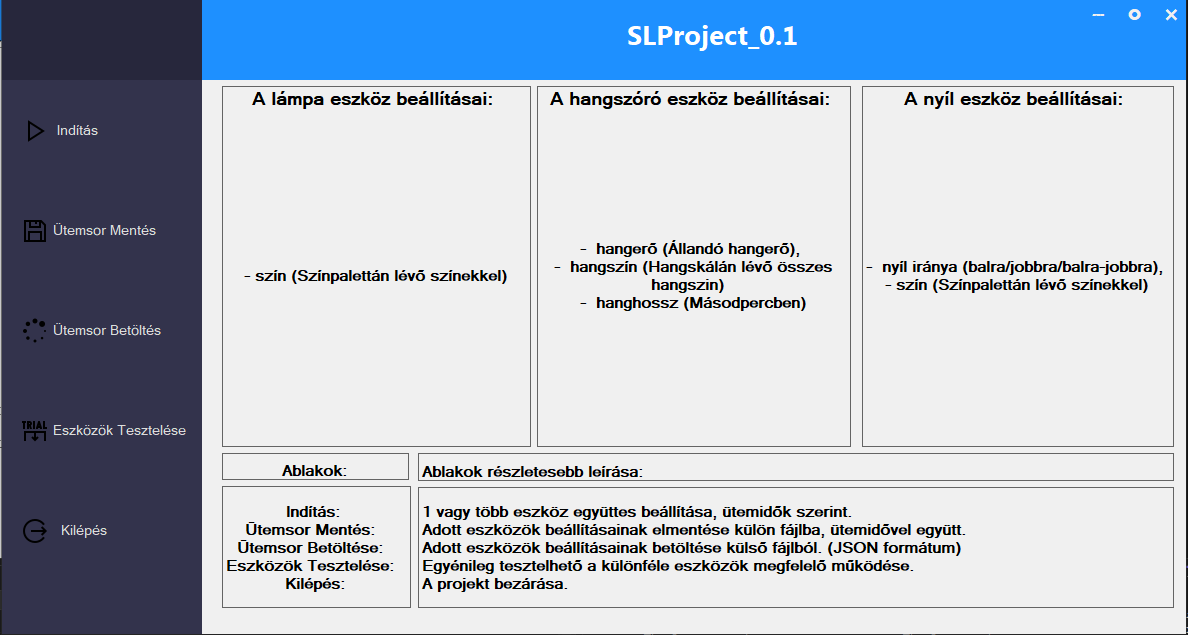
\includegraphics[scale=0.45]{FormMainMenu_land}
		\caption[Kezdő képernyő címkékkel]{Kezdő képernyő címkékkel}
		\label{fig:main_menu_end}
	\end{figure}
	A \ref{fig:main_menu_end} ábrán látható, hogy a kezdőképernyő hordoz magával már információkat arról, hogy az eszközök milyenfajta beállításokkal rendelkeznek. Továbbá, az ablak alsó részében, megtalálhatjuk az oldalsávban lévő gombok leírását is.
	\\
	A következő fejezetekben magát a kezdőképernyőt felépítő kódról szeretnék beszélni.
	\subsubsection{Konstruktor}
	A kezdő menünek a konstruktora sok adatot tartalmaz a formmal kapcsolatban. Alapvetően az első és legfontosabb elem az a \textit{InitializeComponent()} metódus amely az automatikusan megírt kód alapján előkészíti a form képernyőt a különböző objektumok fogadására. Ez a metódus mindegyik Form-nál azonosan szerepel.
	\\
	 A kinézethez nagyban hozzájárult a(z) \textbf{EnableVisualStyles()} nevezetű metódus amely a(z) \textbf{Application} osztály egy metódusa. Az említett metódus akár félreérthető lehet, mivel első gondolatra lehetséges, hogy a fejlesztő arra asszociálhat, hogy a metódus segíti a Form-ban lévő objektumokat, vizuálisan kirajzolni, amely részben igaz. Az előbb említett asszociáció kiegészítve lehet helyes, mivel amikor ez a metódus fut, akkor a beépített Windows rendszer témájától függően alakítja az említett színeket, szövegtípusokat, gombokat, címkéket, és további objektumokat.
	 A színek, betűtípusok és egyéb grafikai elemek együttesen alkotják a felület vizuális stílusát. \cite{enablevisualstyless}
	\subsubsection{panelBeallitas metódus}
	A \textbf{panelBellitas()} metódus egy olyan eljárás amely beállítja a kezdőképernyőhöz tartozó címkéket, amelyek a navigálásnak a leírásáért felelősek. A címkék hozzáfűzését a panelhez, a való Controls.Add() metódussal oldottam meg amely paraméterben vár egy Control objektumot amely jelen esetben számunkra a címkék nevei voltak.
	\\
	Majd miután a címkéket hozzáadtuk a fő panelhez akkor utána a címkéknek a beállításait kell konfigurálnunk a "." operátor segítségével. A "." karakter segítségével betudjuk állítani a címkéink számára a megjelenítendő szöveget, és az ezzel kapcsolatos kinézeti funkciókat.
	\\
	A panelBeallitas eljárást a konstruktorban hívjuk meg.
	\subsubsection{SelectThemeColor metódus}
	A \textbf{SelectThemeColor()} metódus egy olyan függvény amely egy adott oldal fejlécének a színét fogja beállítani. A következő sorokban ezt taglalnám, miként és hogyan teszi ezt. 
	\\
	Elsőnek beállítunk egy index nevezetű változót ami egy véletlenszerűen választott értéket választ a \textbf{SzinTema} nevezetű osztály \textbf{ColorList} listájából. A véletlenszerű kiválasztást a \textbf{Random} osztály \textbf{Next} metódusával érjük el, amely a jelenlegi helyzetben egy 0-tól a \textbf{lista.Count}-ig megy ami a listának a teljes hosszát tartalmazza, vagyis azt, hogy a listában mennyi elem szerepel. 
	\\
	Ezt követően megvizsgáljuk a metóduson kívül létrehozott \textbf{tempIndex} nevezetű értékünket és a most megkapott \textbf{index} nevezetű változónkat, és ameddig a két érték megegyezik egymással addig léptetünk az \textbf{index} változón. Ez a ciklus ez azért szükséges, mivel ha nem létezne ez a lépés akkor első belépésünk után ugyanazokat a színeket kapnánk mindegyik képernyő esetén. 
	\\
	Majd a \textbf{tempIndex} változónkba eltároljuk az \textbf{index} nevezetű változónk értékét, majd ezután a visszatéréshez szükséges \textbf{color} változónkba eltároljuk az \textbf{index} helyen található, szín kódját. Majd az így kapott értékkel térünk vissza, melyet a(z) \textbf{ColorTranslator} osztály \textbf{FromHtml()} nevezetű metódusán keresztül fordítunk át tényleges \textbf{ARGB} színként.
	
	
	\subsubsection{ActivateButton metódus}
	A(z) \textbf{ActivateButton()} paraméterében vár egy \textbf{btnSender} nevezetű objekt típusú változót, emellett visszatérési értéke a metódusnak nincsen. A \textbf{btnSender} változót megvizsgáljuk hogy a benne lévő érték üres-e vagyis \textbf{null} értékkel egyenlő-e vagy sem. Amennyiben van a változóban érték, ekkor megvizsgáljuk hogy a metóduson kívül létrehozott \textbf{currentButton} változónkkal megegyezik-e a paraméterben kapott változó. Amennyiben a két érték nem egyezik akkor meghívjuk a \textbf{DisableButton()} nevezetű metódusunkat amelynek a kifejtését a \ref{Disablebuttonlabel} számú alfejezetben írom le.
	\\
	 Majd ezután egy átmeneti \textbf{color} változóba elmentjük a \textbf{SelectThemeColor()} metódusból származó szín értékét. Ezt követően a \textbf{currentButton} változót beállítjuk a paraméterben kapott változójaként, majd ennek a \textbf{currentButton} változó beállításait konfiguráljuk. Ezt követően a fejléc színét is beállítjuk a kapott \textbf{color} változóra, és a \textbf{SzinTema} nevezetű osztály elsődleges (angolul: primary) változóját beállítjuk a \textbf{color} változóra majd ahhoz illesztve a másodlagos (angolul: secondary) szín értékét beállítjuk a \textbf{ChangeColorBrightness()} nevezetű metódusnak az értékére, melyet a \textbf{color} változó és a korrekció faktor alapján számít ki.
	 \\
	 Végül a gombot amely az alaphelyzetbe állítását végzi a formnak, azt a gombot igazra (angolul:True) állítjuk.
	\subsubsection{DisableButton metódus}
	\label{Disablebuttonlabel}
	A \textbf{DisableButton} metódus azért képezi fontos részét a vizualizációnak mert amikor a felhasználó navigál a gombok között akkor kattintásával megváltoztatja az adott gombnak a háttérszínét is, ezzel elérve azt, hogy tudja a felhasználó, hogy éppen melyik formban tartózkodik. Ez a funkció színesebbé teszi a formot és felhasználó barátibb lesz a rendszer maga. Ebben a metódusban ezt a színváltoztatást úgy érhetjük el, hogy a \textbf{panelMenu}-nek a \textbf{Controls} mezőjét végigjárjuk egy ciklussal és megvizsgáljuk, hogy az adott \textbf{Control} típusú változónak a típusa az gomb-e.
	Amennyiben a bool értéke a feltételnél Igaz abban az esetben az adott gombnak a háttérszínét és szövegtípusát megváltoztatjuk.
	\\
	Ellenkező esetben ha a feltétel kiértékelésénél Hamis értéket kapunk akkor nem változtatjuk meg az adott \textbf{Control} típusú változó értékeit.
	\\ 
	Ez a feltétel kiértékelés azért fontos mivel ha nem vizsgálnánk meg azt hogy az adott \textbf{Control} típusú objektum gomb-e, akkor az összes gombnak a színezése változatlan állapotba maradna.
	\subsubsection{OpenSubForm metódus}
	Az \textbf{OpenSubForm()} metódust arra fogjuk használni, hogy előző formban lévő adatokat, színeket átadjuk a másik következő formnak. Amikor rákattint a felhasználó az adott gombra, akkor ezt az eljárást hívjuk meg melynek paramétereiben megadjuk a kívánt formnak az objektumát, és a \textbf{sender}-t amely a gombnyomás metódus paraméteréből származik. A jelenlegi eljárásban, az éppen aktív formnak értékül adjuk a kattintáskor megadott form értékét. Ezt követően a paraméterben kapott form beállításait változtatjuk, majd megjelenítjük ezen formot. 
	\\
	A \textbf{Form Main Menu}-n kívül az összes másik formot az \textbf{OpenSubForm()} metódussal hívunk meg.
	\subsubsection{Reset metódus}
	A \textbf{Reset} metódus meghívja a \textbf{DisableButton()} nevezetű metódust mely alaphelyzetbe állítja az oldalsávban lévő gombok színét, és stringjük méretét.
	\\
	Ezt követően a címhez tartozó címke \textbf{Text} változóját átírjuk \textbf{HOME}-ra, és mindent alapbeállításokra állítunk. Ezek tartalmazzák a címke átírása mellett a háttérszín alapszínre állítását, illetve a gyermek formot bezáró gomb láthatóságának false-ra vagyis hamisra állítását is.
	\\
	\subsubsection{Gomb Kattintás metódusok}
	Amikor a felhasználó az egyik oldalsávbeli gombra kattint akkor a gomb Click eseménye meghívja az OpenSubForm metódust, amely elvégzi a megfelelő oldalsávbeli gombok színének beállításait, és megnyitja a megfelelő formot.
	\subsubsection{Oldalsáv}
	Az alap formunk még egy oldalsávból is áll a kezdőképernyőnk amely navigációt és könnyebb tájékozódást jelenthet a felhasználó számára.
	Ebben a sávban gombok helyezkednek el amelyeknek, külön hátterük, és ikonjuk van. Ezek mind hozzájárulhatnak a felhasználó-barát szemléletmódhoz. Mindegyik gombhoz tartozik egy esemény amelyben a megfelelő form-ok nyílnak meg.
	\\
	A navigáció sávban megtalálhatjuk a következő gombokat:
	\begin{itemize}
		\item Indítás
		\item Ütemsor Mentés
		\item Ütemsor Betöltés
		\item Eszközök Tesztelése
		\item Kilépés
	\end{itemize}
	Az \textbf{Indítás} gomb a fő formunk az egész alkalmazáson belül, mivel itt tud a felhasználó, különféle ütemenként összeállítani, úgynevezett "gyakorlatokat" amelyek magába foglalják a lámpa, hangszóró és a nyíl eszköz külön működését. A többi információt a fő formmal kapcsolatban majd a \ref{FormInditas} alfejezetben fejteném ki.
	%még nem tom mi kéne ide
	\\
	A  \textbf{Feladatsor Mentés} gombnak a segítségével a jelenlegi eszközöknek a beállításait mentheti el a felhasználó, amennyiben számára az eszközök elérhetőek. A funkció kifejtését és a megoldását a későbbiekben, a Form Mentés \ref{Form Mentes} alfejezetben fejteném ki.
	\\
	A \textbf{Feladatsor Betöltés} gomb használatával a felhasználó képes betölteni adott eszközökhöz tárolt adatokat, mint például: adott lámpákhoz tartozó LED-ek színét, vagy adott nyilakat ábrázoló eszközöknek a színét illetve irányát, vagy esetlegesen a hangszínt, és még a hanghosszt adott hangszórók esetén.	Ezeknek kifejtését a Form Betöltés című \ref{Form Betoltes}
	alfejezetben fejtem ki.
	\\
	A \textbf{Feladatsor Szerkesztés} gomb használatával a felhasználó tudja szerkeszteni a már ismert eszközöket, és mint egy "demo" változatot kipróbálhatja az eszközök működését. Ezeknek a kifejtését a Form Szerkesztés című \ref{Form Szerkesztes}	alfejezetben fejtem ki.
	\\
	A \textbf{Kilépés} gombot arra használhatja a felhasználó, hogy az alkalmazást terminálni tudja. A kilépés gomb eseményéhez kötöttem egy Exit() metódust ami az Application osztálynak az egyik metódusa. Ez a metódus bezárja az applikációt, és befejezi a program futását. 
	\\ 

	\subsection{Form Inditás}
	\label{FormInditas}
	Az "Indítás" nevezetű oldalsávbeli gombra kattintva elérhetjük az alkalmazásunk fő ablakát, amely arra hivatott, hogy a projekt fő célját elvégezze: Vagyis, hogy a birtokunkba lévő eszközöket, legyen az lámpa, nyilat ábrázoló lámpa, vagy hangszóró, tudjunk vezérelni külön is meg akár egyben is.
	Lehetősége van a felhasználónak, új sort/ütemet hozzáadni a jelenlegi eszközeihez. Ezen felül még minden egyes eszközt külön tud szerkeszteni, amely által színesebbé teheti az ütemek lejátszását.
	Az ütemek timer-hez vannak kötve, amelyet a felhasználó be tud konfigurálni
	A projekt jelenleg képes 1 vagy 2 eszköz együttes működtetésére, amelyek kombinációjával sokféle színes gyakorlatokat tudunk felépíteni.
	\\
	\subsubsection{Felmerülő problémák a panel vezérlővel}
	Eleinte a fő ablak kidolgozása is problémákkal kezdődött, mivel felmerült az, hogy az eszközöket amelyeket észlel a DLL-ből kapott program, hogyan jelenítsük meg? Erre elsősorban a panel objektum tűnt megfelelőnek. A \ref{fig:prototipus1} ábrán láthatjuk a főképernyőt a panelek felhasználásával.
	\begin{figure}[H]	
		\centering
		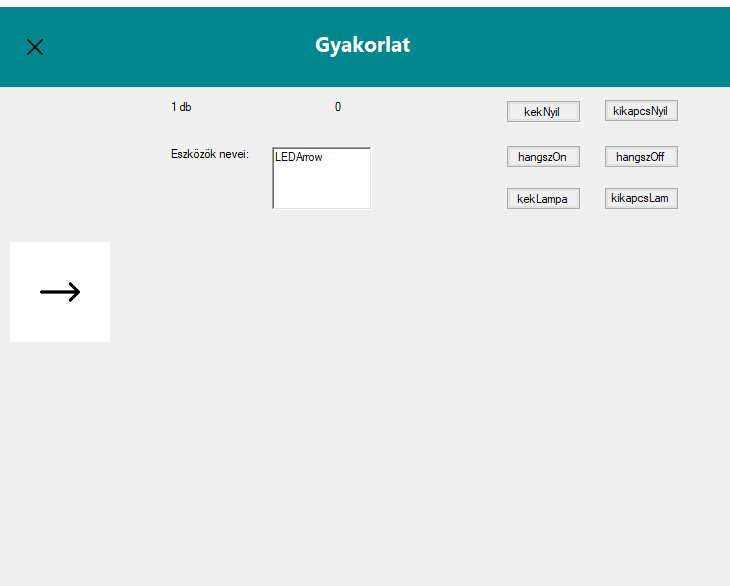
\includegraphics[scale=0.5]{prototípus1}
		\caption[Indítás képernyő panelekkel megoldva]{Indítás képernyő panelekkel megoldva}
		\label{fig:prototipus1}
	\end{figure}
	A panel egy olyan konténeres vezérlő, amelyben hasonló "gyermekvezérlőket" is lehet elhelyezni. \cite{panelc}
	A panelbe könnyedén el lehet helyezni gombokat, szövegdobozokat, és más különböző objektumokat is, de ezen objektumokat nehéz volt megkülönböztetni. 
	\subsubsection{Panel vezérlő kiváltása DataGridView segítségével}
	A DataGridView vezérlő azért megfelelő választás viszonylag rugalmas módot biztosít az adatok táblázatos formában történő megjelenítésére.\cite{datagridc} 
	A DataGridView vezérlő emellett azért is bizonyult jobbnak mint a Panel vezérlő, mivel a DataGridView sorokkal és oszlopokkal van felépítve, amelyek interszekciója, egy cellát épít fel, amely jelen esetben számunkra egy gomb lesz. Így ezentúl tudunk erre a cellára hivatkozni, és képesek vagyunk megkülönböztetni őket.
	A végső kinézete a főablaknak a \ref{fig:inditas3eszk} ábrán található.
	A következőkben a fő formnak a metódusairól szeretnék bővebben írni.
	\begin{figure}[H]	
		\centering
		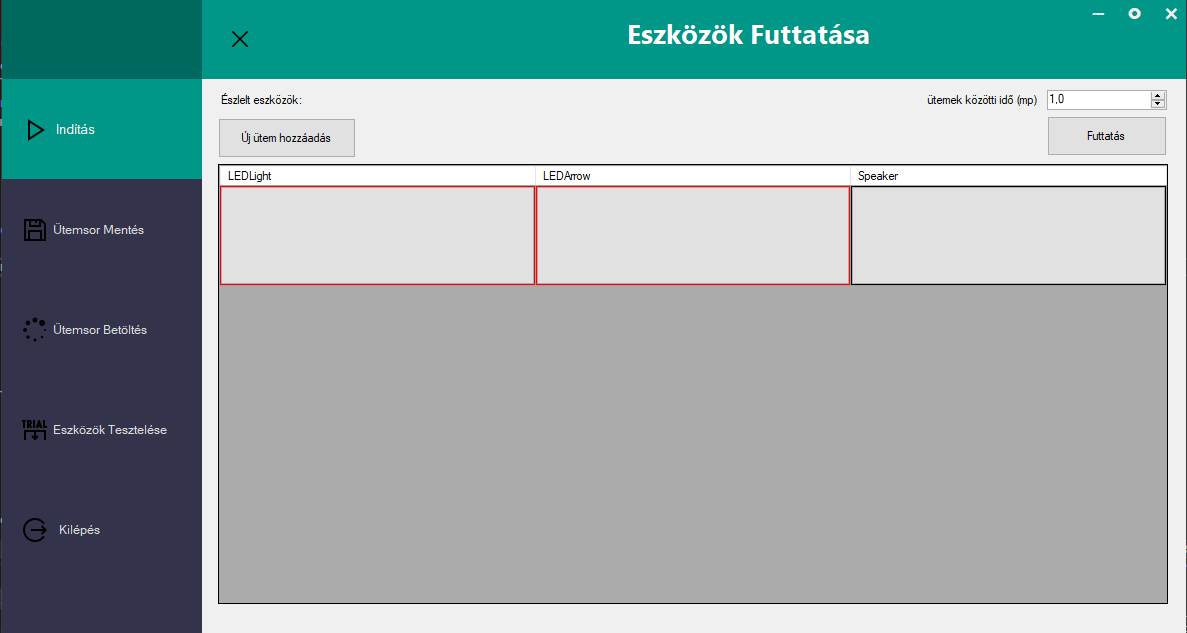
\includegraphics[scale=0.5]{Form_inditas_3eszkoz}
		\caption[Indítás képernyő 3 eszközzel]{Indítás képernyő 3 eszközzel}
		\label{fig:inditas3eszk}
	\end{figure}
	\subsubsection{Konstruktor}
	A form konstruktorában hasonló módon jelennek meg a metódusok, mint a FormMainMenu-ben is, azzal a kivétellel, hogy a DataGridView vezérlő inicializálást végző eljárást is meghívjuk, mivel a form betöltésekor kell lefutnia. Ennek oka, hogy a gombokat és a különböző címkéket helyesen, és jól megjelenítse a képernyő.
	\subsubsection{DataGridViewBetolt metódus}
	A DataGridViewBetolt eljárás a DataGridView vezérlő alap konfigurációit végzi el. Ebbe beletartozik a vezérlő méretének beállítása, az hogy görgethető lehessen a vezérlő, és legutolsó sorban az, hogy helyes módon jelenítse meg az eszközöket szimbolizáló gombokat. 
	\\
	Minden egyes oszlophoz van rendelve egy HeaderText érték amely az adott eszköz oszlopát jeleníti meg ezzel, segítve a felhasználót. Továbbá, csak annyi eszköz jelenik meg a vezérlőn belül amennyit éppen érzékel a program, és ezen érzékelés alapján jelenít meg annyi gombot amennyi szükséges. 
	\subsubsection{utemTimer\_Tick metódus}
	A tick eljárás, a Timer-nek az eseménye, amely mindig lefut ha eltelik egy adott idő amelyet értéket megadunk futásidőben. Ebben az eljárásban, beállítjuk az eszközöket a felhasználó által kapott értékekre. Ezt követően pedig amikor egy újabb "Tick" következik akkor beállítjuk a következő sorban lévő értékekre az eszközöket.
	\subsubsection{jsonBeMentes metódus}
	Mivel az ütemek kitöltését futási időben kell megoldanunk ezért a legmegfelelőbb módszer az volt, hogyha a jelenlegi form-ban írom meg ezen metódusokat.
	A jsonBeMentes eljárás paraméterbe kap egy stringet amely a fájl kimentésének a helyét határozza meg. Ezentúl az eljárásban szerepel egy SerializedTurnSettings tömbböt amelyet a DLL-ből kapunk meg. Ennek a tömbnek a mérete az oszlopok száma. Majd ezt egy iteráció követi amely végigjárja a GridView-nak az oszlopait és ebben a ciklusban megkapjuk az eszközök beállításait.
	Majd ezeket követően JSON formátumra alakítjuk az eszközök beállításait, és kiíratjuk a beállításokat a File.WriteAllText() nevezetű metódussal.
	
	\subsubsection{jsonBolBetoltes metódus}
	
	A betöltés nehezebbnek bizonyult, mint a mentés mivel, itt a JSON formátumú fájlból kell kikérnünk a beállításokat.
	Ehhez megoldásként a DLL-ből kapott LoadDeviceSettings függvényt használtam fel, amelybe a JSON fájlt alakítja át és helyezi bele az eszközökbe, mint konfigurációt. Majd ezt követően már be lehetett állítani azt, hogy mennyi oszlopot és sort generáltassunk le a DataGridView-ban a FormHelper.Devices.Count segítségével.
	
	\subsubsection{dataGridInditas\_CellContentClick metódus}
	Ezen eljárás egy kattintás esemény, amely akkor fut le, hogyha az adott cellára/gombra rákattint a felhasználó.
	Amikor ez megtörténik, akkor a program megvizsgálja, hogy az adott cellában lévő gomb az valójában beletartozik-e az eszközök csoportjába, és amennyiben igen, akkor a helyes szerkesztési formot jeleníti meg a felhasználónak, egy apró felületen keresztül.
	
	
	\subsection{Form Mentés}
	\label{Form Mentes}
	 Alapvetően, a mentés form arra lesz hivatott, hogy a SaveFileDialog nevezetű osztályt felhasználva a megfelelő helyre mentse ki a JSON fájlt. A form képes jelenleg mindegyik eszköz beállításainak kimentésére. Egy JSON formátumú fájlba való kimentés a \ref{fig:keteszkozkimentes} ábrán található.
	 \begin{figure}[H]	
	 	\centering
	 	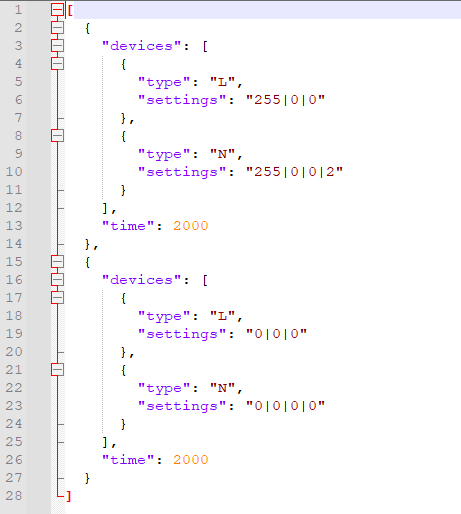
\includegraphics[scale=0.7]{két_eszköz_kimentésének_a_JSON_fájlja}
	 	\caption[Kimentés, JSON fájlba lámpa és nyíl eszközzel]{Kimentés, JSON fájlba lámpa és nyíl eszközzel}
	 	\label{fig:keteszkozkimentes}
	 \end{figure}

	A JSON azért optimális fájl formátum mivel közismert és tökéletes arra, hogy átmeneti adatot tároljunk benne. 
	\\
	Ilyen átmeneti adat lehet egy felhasználó által generált adat, vagy például a jelenlegi helyzetben az eszközök beállításai. 
	\\
	A mentést a \textbf{Feladatsor Mentése} gomb megnyomásával válthatja ki a felhasználó. Ezt követően pedig ki kell választania a felhasználónak, hogy hova szeretné elmenteni a \textbf{JSON} fájlban eltárolt eszközök adatait.
	A mentésről videofelvétel \url{https://youtu.be/0YGDGnBJYLA} linken találhatunk felvételt.
	\\
	A mentés azért is lehet optimális funkció mert ha a későbbiekben szükségünk volna egy adott beállításra, akkor lementjük az eszközök adatait és amikor újra szükségünk lesz betöltjük azokat a \textbf{Feladatsorok Betöltése} gombbal. Későbbiekben a betöltésről a \ref{Form Betoltes}
	\subsubsection{Konstruktor}
	A mentés formnak a konstruktora hasonlóképpen épül fel mint a \ref{FormMainmenu} fejezetben lévő konstruktor is. 
	Miután meghívtuk a \textbf{LoadTheme()} metódust utána a \textbf{Mentes()} nevezetű eljárást hívjuk meg amely magát a fájl mentésének a helyét választja ki és ehhez a SaveFileDialog osztályt használja fel. Erről a metódusról későbbi alfejezetben írnék.
	Továbbá, meghívjuk még a konstruktor paraméterében kapott FormInditas által meghívott jsonBeMentes() metódust is amelynek paraméterében a kimentés stringjét adjuk át. A \textbf{jsonBeMentes()} metódusról a \ref{FormInditas} fejezetben írtam le részletesebb információkat.
	\subsubsection{Mentes metódus}
	A \textbf{Mentes()} metódus számunkra ebben a formban a legfontosabb lesz mivel ez alakítja a \textbf{FormMentes}-nek a lényegét. 
	\\
	A mentéshez az úgynevezett \textbf{SaveFileDialog} nevezetű osztályt fogjuk használni. 
	\\
	Amikor a felhasználó elszeretne menteni egy vagy esetlegesen több eszköznek a beállításait akkor a \textbf{SaveFileDialog} segít kiválasztani a mentési helyet és a fájlnevet is. Hasonló a működése az \textbf{OpenFileDialog}-hoz amelyet a betöltés formnál fogunk használni. A \textbf{SaveFileDialog} egy általános Windows "párbeszédpanel" burkolatba van becsomagolva ami lehetővé teszi azt, hogy a felhasználó tudjon kommunikálni a rendszerrel.
	\\
	A legelső lépés ahhoz, hogy elérjük azt, hogy menteni lehessen, kell számunkra egy új példány a \textbf{SaveFileDialog}-ból. Ezt követően pedig beállíthatunk néhány opcionális beállítást. Ilyenek például az, hogy amikor megnyitja a felhasználó a mentést akkor melyik könyvtárból induljon ki a kezdeti megnyitáskor. 
	\\
	Lehetséges \textbf{Filtereket}, szűrőket is hozzáadni az opciókhoz amelyek segítségével bebiztosíthatjuk a programunkat, hogy csakis \textbf{JSON} fájlokat tudjon elmenteni.
	\\
	Ezt követően megvizsgáljuk, hogy a felhasználó az \textbf{OK} gombra nyomott-e és nem szakította meg a mentés folyamatát. Amennyiben a mentés során minden lefutott akkor elmentjük a fájl elérési útját amelyet később a konstruktorban lévő \textbf{jsonBeMentes()} metódus kapja meg.
	A mentés gomb a \ref{fig:mentesgomb} ábrán látható.
	\begin{figure}[H]	
		\centering
		\includegraphics[scale=0.5]{Ütemsor_ment}
		\caption[Mentés ablak elhelyezkedése az oldalsávon]{Mentés ablak elhelyezkedése az oldalsávon}
		\label{fig:mentesgomb}
	\end{figure}
	\subsection{Form Betöltés}
	\label{Form Betoltes}
	A feladatsorok vagyis az eszközök beállításához tartózó konfigurációkat meghívó formot is a \textbf{OpenSubForm()} nevezetű metóduson hívunk meg. A betöltés form célja az, hogy eszközök alapján amelyek éppen csatlakoztatva vannak a rendszerünkhöz, betöltsünk hozzájuk egy adott konfigurációt.
	Jelenleg ez a funkció egyéni eszközök beállításainak betöltésére alkalmas.
	\\
	Ezen konfigurációkat, úgy tudjuk betölteni, hogyha van, egy vagy több eszközbeállításokat tartalmazó JSON fájlunk, amelyet be tud tölteni a rendszer. Ezt a betöltést a \ref{FormInditas} fejezetben található \textbf{jsonBolBetoltes()} metódus végzi el
	\subsubsection{Konstruktor}
	A betöltés formnak a konstruktora vagyis a belépési pontjában megtalálhatjuk a \textbf{Betoltes()} nevezetű eljárást amely magát a fájl betöltését végzi el. Erről a metódusról későbbi alfejezetben írnék.
	\subsubsection{Betoltes metódus}
	A \textbf{Betoltes()} metódus kicsit máshogyan fog kinézni mint a \ref{Form Mentes} fejezetben lévő \textbf{Mentes()} metódus. Ezen metódus képezi a Betöltés magját, mivel itt érhetjük el, hogy betudjunk tölteni a JSON fájlt.
	\\
	A betöltés algoritmusához a(z) \textbf{OpenFileDialog} nevezetű osztályból fogunk használni metódusokat és mezőket. Hasonló módon mint a \textbf{SaveFileDialog} osztálynál itt sem tudunk örökölni ebből az osztályból ezért ahhoz, hogy tudjuk a \textbf{public} láthatósági szinttel ellátott metódusait és objektumait használni ezért szükségünk lesz az osztály objektumára.
	Ehhez meghívjuk az \textbf{OpenFileDialog} osztályt, és egy objektumán keresztül hívogatjuk meg a publikus metódusait és mezőit.
	\\
	Ezek után az \textbf{InitialDirectory}-t vagyis a kezdő könyvtárat állítjuk be, mely a felhasználót a gomb megnyomásakor az adott könyvtárba helyezi el. Ebből a könyvtárból tud navigálni tovább, és keresheti meg a betölteni kívánt fájlt. 
	\\
	Majd a további beállítások a \textbf{Filter} mely segít abban, hogy csak azokat a fájlokat tudja leszűrni amelyeket tud fogadni a rendszer.
	És még más további beállításokat is tudunk konfigurálni.
	\\
	A beállításokat követően megvizsgáljuk, hogy a felhasználó sikeresen  megtalálta-e a JSON fájlt. Amennyiben helyesen megtalálta a fájlt utána elmentjük egy változóba a fájl nevét.
	\\
	Ezután átadjuk ezt az értéket a konstruktorban lévő \textbf{jsonBolBetoltes()} metódusnak a paraméterében.
	És a betöltéshez tartozó gombok megjelenítését a jsonBolBetoltes metódusra bízzuk rá.
	A betöltés gomb a \ref{fig:betoltesgomb} ábrán látható.
	\begin{figure}[H]	
		\centering
		\includegraphics[scale=0.5]{Ütemsor_betolt}
		\caption[Betöltés ablak elhelyezkedése az oldalsávon]{Betöltés ablak elhelyezkedése az oldalsávon}
		\label{fig:betoltesgomb}
	\end{figure}
	
	
	\subsection{Form Szerkesztés}
	\label{Form Szerkesztes}
	Az eszközökhöz tartozó szerkesztés képernyőt ebben a formban jelenítjük meg. A felhasználó ezen képernyőn kipróbálhatja az eszközeit, hogy mindegyik működik-e megfelelően vagy sem. Ehhez a formhoz szükségünk lesz még több formra is, amelyek ilyen alképernyőként funkcionálnak majd programunkban.
	\\
	A jelenlegi szerkesztés képernyőből fogunk navigálni attól függően, hogy éppen milyen eszköz van csatlakoztatva a rendszerbe. A szerkesztés formról képet a \ref{fig:SzerkformFo} ábrán találhatunk.
	\begin{figure}[H]	
		\centering
		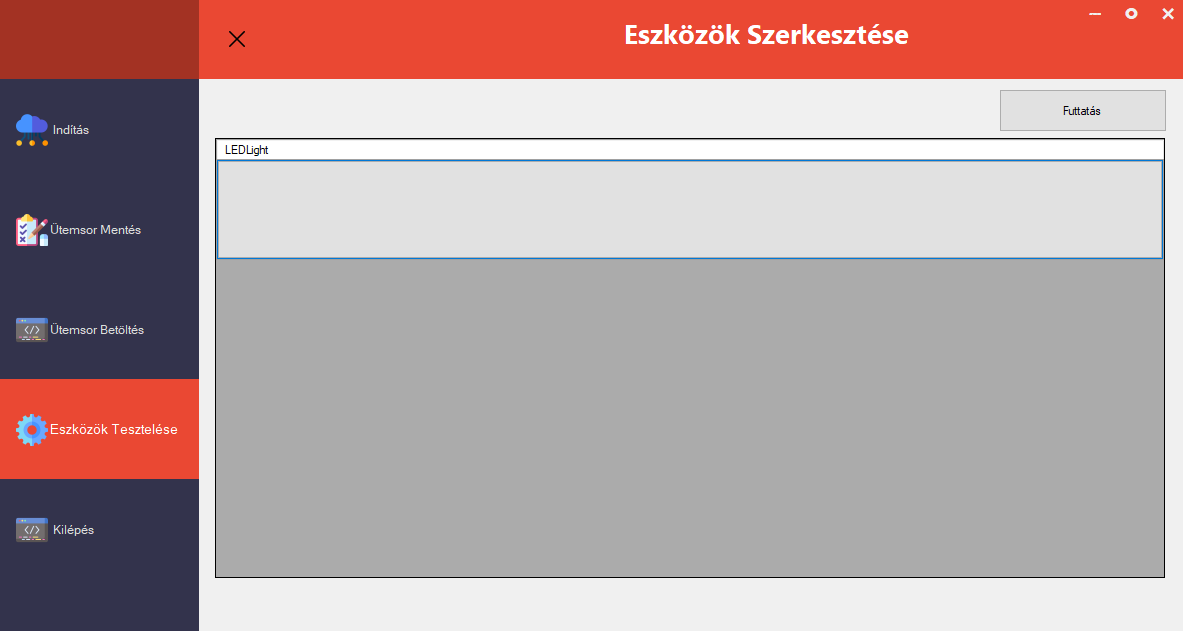
\includegraphics[scale=0.5]{FormSzerk_page}
		\caption[Szerkesztés Form Fő ablaka]{Szerkesztés Form Fő ablaka}
		\label{fig:SzerkformFo}
	\end{figure}
	A kód felépítése a következő alfejezetekben lesz tárgyalva.
	\subsubsection{Konstruktor}
	A főszerkesztés formnak a konstruktora, vagyis a belépési pontjában megtalálhatunk hasonlóságokat az előző formokkal együtt nézve.
	Ebben a formban is mint az Indítás formban egyaránt DataGridView vezérlővel fogunk dolgozni, amelynek hasonlóképpen állítjuk be a konfigurációit, mint az Indítás formban. A beállításokat a \ref{FormInditas} fejezet Konstruktor alfejezetében találhatjuk meg.
	\subsubsection{dataGridSzerkesztes\_CellContentClick metódus}
	Ezen metódusban hasonlóképpen mint az Indítás formban, a DataGridView-ban lévő cellák értékeit vizsgáljuk meg, és az alapján, hogy az adott cella milyen típusú úgy nyitja meg az eszközhöz tartozó  szerkesztést. Háromféle eszköz szerkesztése lehetséges: a lámpa, nyíl, hangszóró.
	\subsubsection{btnFuttatasSzerk\_Click metódus}
	A futtatás szerkesztés kattint esemény, akkor fut le amint a felhasználó a "Futtatás" gombra kattint, ekkor az eszközöket megvizsgálja, és beállítja azokat a megfelelő beállításra amelyet a felhasználó adott meg. Az eljárás algoritmusa az \ref{alg:cap} ábrán található.
	\begin{algorithm}
		\caption{Eszközök beállítása a szerkesztés formban}\label{alg:cap}
		\begin{algorithmic}
			\Procedure{btnFuttatasSzerk\_Click}{ }
				\If{$ledLight1 \! \neq \!null$}
				\\
				$\qquad \qquad \qquad $ ledLight1.Color = FormLampaSzerk.colors[0] //lámpa színe beáll.
				\EndIf
				\If{$ledArrow1 \! \neq \!null$}
					\\
				$\qquad \qquad  \qquad $ ledArrow1.Color = FormNyilSzerk.colors[0] // beállítjuk a nyíl színét.
				\\
				$\qquad \qquad  \qquad $  ledArrow1.Direction = FormNyilSzerk.directions[0] // nyíl irány beáll.
				\EndIf
				\If{$speaker1 \! \neq \!null$}
					\\
				$\qquad $ speaker1.AddSound(FormHangszSzerk.pitch[0],63, FormHangszSzerk.timeMilisec[0])$\qquad $// beállítjuk a hangszóró adatait.
				\EndIf
				\\
				 string json\_source = FormHelper.DevicesToJSON(); $\qquad $// JSON-né alakítás
				 \\
				  FormHelper.CallSetTurnForEachDevice(ref json\_source);$\qquad $// beállítás kiküldése
				 \\
				 \If{$speaker1 \! \neq \!null$}
				 \\
				 $\qquad \qquad  \qquad $ 
				 speaker1.ClearSounds(); $\qquad $// a speakert alapra állítjuk
				 \EndIf
			\EndProcedure
		\end{algorithmic}
	\end{algorithm}
\\
	A következő három fejezetben a különféle eszközökhöz tartozó form kialakításáról lesz szó.

	\subsection{Form Hangszóró Szerkesztés}
	A különböző eszközökhöz tartozó szerkesztési formokat, külön képernyő segítségével oldottuk meg, amelyek mint egyfajta \textit{"gyermek"} form-ként is szolgálnak az előző \ref{Form Szerkesztes} fejezet számára. 
	
	

	A hangszóró form, a hangszóró eszköznek a szerkesztésére alkalmas képernyő, ahol az adott hangszóróhoz tartozó beállításokat állíthatjuk be. A kezdeti megvalósításban a képernyő a \ref{fig:hangszformProb} ábrán látható módon tűnt fel.
	 \begin{figure}[H]	
		\centering
		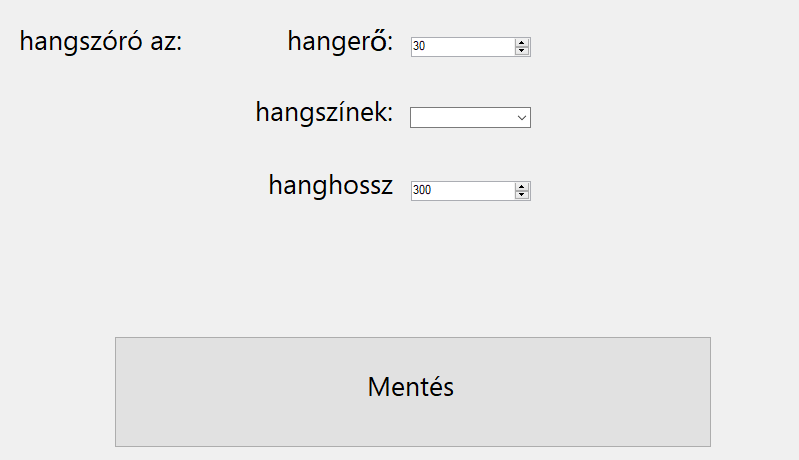
\includegraphics[page=1,width=0.5\textwidth]{hangsz_form}
		\caption[Hangszóró form prototípusa]{Hangszóró form prototípusa}
		\label{fig:hangszformProb}
	\end{figure}
	A további fejlesztések során felmerült annak igénye, hogy egyes eszközök szerkesztési képernyője ne tűnjön nagynak, hanem inkább legyen esztétikailag egyszerű. Ezen okból kifolyólag át lett alakítva a form teljesen ahogyan azt a \ref{fig:hangszFormFo}.
	\begin{figure}[H]	
		\centering
		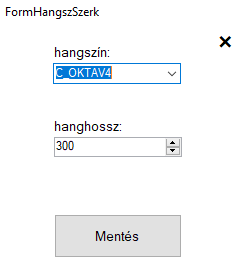
\includegraphics[page=1,width=0.4\textwidth]{hangsz_szerk}
		\caption[Hangszóró form legutolsó kinézete]{Hangszóró form legutolsó kinézete}
		\label{fig:hangszFormFo}
	\end{figure}
	Az utóbbi leegyszerűsített változat, letisztultabb, és kevesebb hely is található rajta, amely segíti a felhasználót az egyszerű átláthatóságban. 
	A képernyőn beállíthatjuk a hangszínt, és hanghosszt.
	A hangszínt beállítását a legördülő mező segítségével érhetjük el. A beállítani kívánt hangszínt kiválasztva, megtudjuk adni azt is, hogy hány másodpercig játssza le azt a bizonyos hangszínt amit kiválasztottunk.
	\\
	A hanghossz értékét betudjuk állítani milliszekundumban is ezért ha például 0,5 másodpercig szeretnénk, hogy hangozzon az adott hangszín amit megadunk az eszközünknek akkor 0,5 értékre kell beállítanunk a hanghossz változót.
	\\
	Miután be lettek állítva a mezők értékei a "Mentés" gombra kattintva, beállítottuk a hangszóró eszközünknek a konfigurációit.
	\newpage
	\subsection{Form Lámpa Szerkesztés}
	A lámpa form, a lámpa eszköz paramétereit konfigurálja be. Eleinte a form a \ref{fig:lampaformKezd} módon volt látható.
	\begin{figure}[H]	
		\centering
		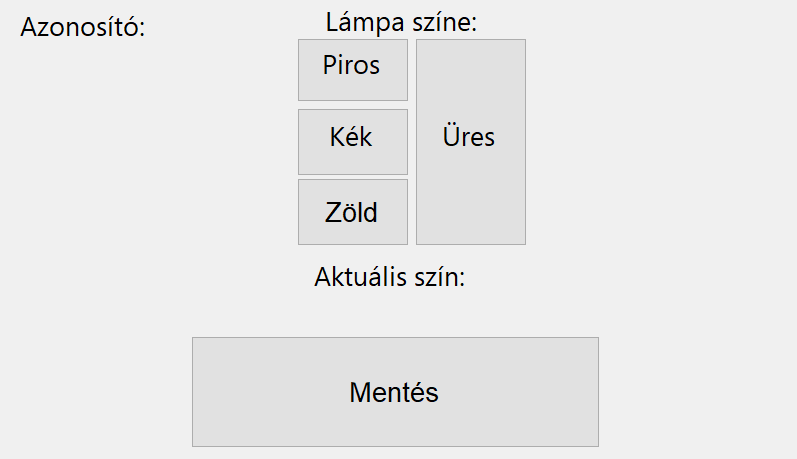
\includegraphics[page=1,width=0.5\textwidth]{lamp_form}
		\caption[Lámpa form kezdeti állapotban]{Lámpa form kezdeti állapotban}
		\label{fig:lampaformKezd}
	\end{figure}
	Mivel ez a kialakítás túl sok helyet ölelt fel, és a színek beállításai le voltak redukálva, piros, kék, és zöld színre ezért egy másikfajta megoldást kellett találnom a probléma kiiktatására.
	Kutatást követően találtam egy úgynevezett \textbf{ColorPickerBox} objektumot, amely mintegy színpaletta segít kiválasztani különböző színárnyalatokat. A ColorPickerBox megvalósítást a nyíl eszköznél is alkalmaztam.
	Egy kis formázás után a formunk a \ref{fig:lampaformveg} ábrán látható módon néz ki.
	\begin{figure}[H]	
		\centering
		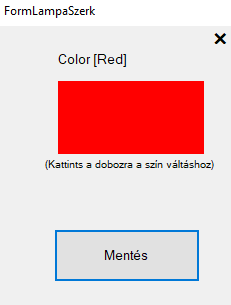
\includegraphics[page=1,width=0.4\textwidth]{LampaSzerk}
		\caption[Lámpa form legutolsó kinézete]{Lámpa form legutolsó kinézete}
		\label{fig:lampaformveg}
	\end{figure}
	Miután kiválasztottuk a megfelelő színt számunkra, utána a Mentés gombbal tudjuk azt ellenőrizni, hogy a lámpánk valóban helyes jelet kap.
	\subsection{Form Nyíl Szerkesztés}
	A nyíl form, a nyíl eszköz paramétereit konfigurálja be. Eleinte a form a \ref{fig:nyilformKezd} módon volt látható.
	\begin{figure}[h!]	
		\centering
		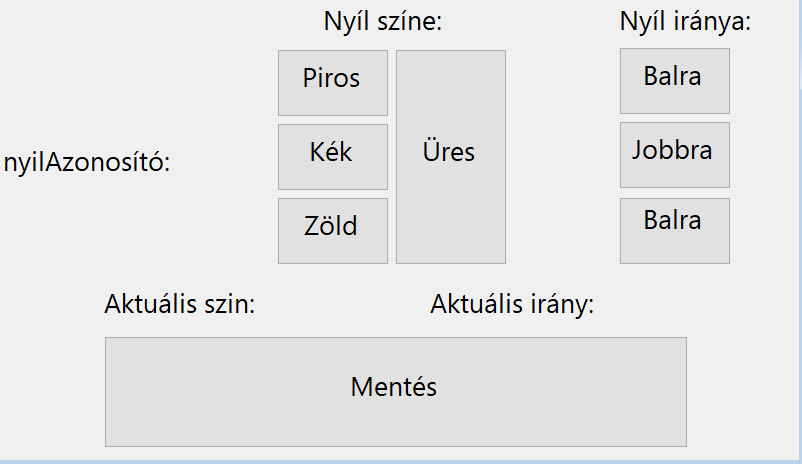
\includegraphics[page=1,width=0.5\textwidth]{nyíl_form}
		\caption[Nyíl form kezdeti nézete]{Nyíl form kezdeti nézete}
		\label{fig:nyilformKezd}
	\end{figure}
	A nyíl formnál is felmerültek hasonló problémák mint az előzőeknél is. A kialakítás túlságosan rendezetlen volt, és ugyanúgy mint a lámpánál is csak háromféle színt lehetett beállítani.
	Ezért felhasználjuk a ColorPickerBox-ot és ennek segítségével választjuk ki a megfelelő színárnyalatot. Továbbá, a nyíl irányának kiválasztását se szövegesen jelenítjük meg hanem mint ábra.
	A végső kinézete a képernyőnek az alábbi módon lett megvalósítva:
		\begin{figure}[h!]	
		\centering
		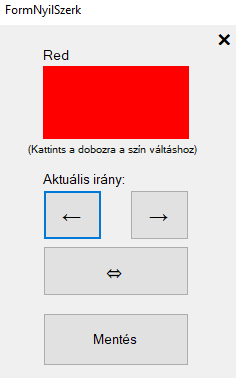
\includegraphics[page=1,width=0.4\textwidth]{nyilSzerk}
		\caption[Nyíl eszközhöz szerkesztési form]{Nyíl eszközhöz tartozó szerkesztési form}
		\label{fig:nyilformveg}
	\end{figure}
	Miután beállítjuk a nekünk tetsző színárnyalatot utána betudjuk állítani a nyíl irányát is.
	A nyíl irányát, balra, jobbra, vagy akár mindkét irányba be tudjuk állítani.
	Ezen beállítás annyit jelent az eszköz számára, hogy a nyílban lévő LED-ek más pozícióban kapnak feszültséget.
	\\
	A nyilak ellenőrzésére a \textit{Mentés} gombot kell lenyomni, amely egy esemény hatására, a nyíl eszköznek kiküldi a megfelelő konfigurációkat.
	A nyíl szerkesztési formmal bezárólag az összes form bemutatása megtörtént.

	\chapter*{Kitekintés}
	A rendszer amit kiépítettünk, egyedülálló mivel a hardveres háttere specifikusan épül fel, vagyis nem elterjedt eszközökkel dolgoztunk. Az alkalmazás a non-verbális eszközök palettáját bővítheti a technika segítségével. 
	\\
	Eszközök felhasználására további ötlet, az eszközök felhasználására, akár az lehetne, hogy mintegy közlekedési lámpa szimulálásaként, három lámpa egységes összekötéséből, vezérléséből állna össze. 
	\\
	Bővíthető lenne olyan módon is, hogy egy hangszóróval megtoldva hangjelzéses, átkelő lámpát is tudnánk ezzel szimulálni. Ez így akár a látási nehézségekkel küzdő embereknek is segítséget nyújthat a zebrák átkelése során.
	\\
	Rajtjelző eszköznek is működtethető lenne! Amennyiben késleltetéseket építünk bele a programba, és 3 lámpának a színét egységesen állítunk be, akár felhasználható lehetne ilyen módon is. 
	\\
	A nyíl eszköz egy további felhasználása lehetne! Azáltal, hogy az irányjelző táblákon iránymutatóként funkcionáljon.
	\\
	Mindezek az ötletek jelenlegi projektnek nem képezik szerves részét, de jövőbeni használatra, és továbbfejlesztésre, mindenképpen alkalmas lehet.
	
	
	
	\begin{comment}
		4.fejezet: (future works) továbbiakban milyen kimenetele lesz, ebből szabadalom lesz, az ötletgazda szeretné ezt kiadni olyan módon hogy piaci termék legyen. 
		- Teljesen más technológia
	\end{comment}
	\chapter*{Befejezés}
	Jelenlegi projekt során ablakos applikációt tudtunk készíteni, amely segítségével három fajta eszközt tudunk vezérelni akár önállóan egy eszközt, vagy kettőt együttesen.  
	\par
	A projekt kezdete során jó néhány problémára kellett megoldást találni, amely a megfelelő dizájn kialakítását vagy az eszközök megfelelő megjelenítését jelentik. Célom volt, hogy az alkalmazáson belül egy olyan felületet tervezzek meg, amely dinamikusan megtudja jeleníteni az eszközöket, gombok formájában. Továbbá, kompatibilissé is szerettem volna tenni az alkalmazást, olyan emberek számára is akik, az informatika világában nem jártasak. Az eszközöket tudjuk működtetni C\# ablakos alkalmazáson belül.
	\par
	Azzal a céllal készítettem ezt az alkalmazást, hogy későbbiek során felhasználásra kerüljön. Törekedtem arra, hogy a projekt elkészítésével segíthessem a mozgásfejlesztésre szakosodott szakemberek munkáját.
	\par
	A projekt továbbfejlesztésre alkalmas, akár a meglévő eszközökön túl még több hardveres eszközre is kidolgozható a programkódom alapján, akár más programozási nyelvben is.
	\\
	Örömömre szolgált, hogy egy olyan csapatban dolgozhattam és annak része lehettem amely eredményesen együtt dolgozott a projekt megvalósításában. Dolgozatom során az egészségfejlesztés világát is érintettük, tapasztalatot nyerhettem, hogy hogyan lehet az informatikai tudásomat felhasználni az emberek életminőségének javítására. Somodi László szakedző gondolatain keresztül is sok motivációt kaptam, valamint \textit{,,Mozgáskoordináció- és gyorsaságfejlesztő gyakorlatok óvodától a felnőtt korig''} című alkotásában leírtakból.
	
	Személy szerint kihívásként éltem meg a projektbe való kutatást és programozást, amely segítségre lehet másoknak. Az informatikával mint tudománnyal képesek vagyunk segíteni embertársainkon legjobb tudásunk szerint, amellyel az Isten megáldott bennünket.
	
	Örömömre szolgált, hogy Somodi László szakedző minket kért meg, az elméleteit felhasználva, egy szoftveres háttér kidolgozására. Szakdolgozatunk nem csupán arról szól, hogy amit megtanultunk a gyakorlatban alkalmazzuk, hanem arról, hogy a projekt egy kézzel fogható és hasznos produktum alapja lett.
	
	Munkánkat interdiszciplináris kutatómunka segítette elő, ezen okból kifolyólag érintettünk más és más tudományokat is az informatikán kívül, ideértve a fizikát, és az egészségügyet.
	
	A programozási elméletet és ennek gyakorlati vonatkozásait segítette, Dr. Király Roland  egyetemi docens. A projekt elindulásában, az alapprogramnak a felépítését és struktúráját, ő tervezte meg. Konzultációk során is készségesen segített ötleteket továbbfejleszteni és azt a program szerves részévé tenni. 
	Csapatmunkánk alapját képezte az ő szaktudása.

	\begin{comment}
		Mint minden szoftverre és emberi termékre jellemző, a megoldásaink természetesen nem mondhatóak tökéletesnek, programunk épp annyira időnként karbantartásra és további fejlesztésekre szorulhat. Érdekes volt felfedezni a gRPC és a Proto-nyelv kapcsán a \ref{grpc} fejezetben, hogy ötször-hatszor jobb teljesítmény érhető el az adatok bináris módon történő szerializációjával a szöveges formátumokhoz képest -- jelen állás szerint mégis az utóbbi megoldás számít elterjedtebbnek --, én azt gondolom, hogy mindenképp érdemes lenne munkánkat esetleg egy másik szakdolgozat keretein belül a gRPC irányába elmozdítani.
	\end{comment}

	\chapter*{Köszönetnyílvánítás}
	Szeretném köszönetemet ezúton is kifejezni a konzulensemnek, Dr.Király Roland Egyetemi Docens úrnak, aki lehetővé tette a téma kidolgozását.
	Szakértelme és tudása nagyban segítette szakdolgozatom programjának sikeres megvalósítását.
	\\
    Köszönettel tartozom Somodi László UEFA "A" licences labdarúgó szakedző úrnak, azért a motivációt amit könyvével és gyakorlati tapasztalatával adott a szakdolgozat megírásához. 
	\\
	Továbbá, szeretném megköszönni, kedves barátomnak és szaktársamnak, Nagy-Tóth Bencének is a sok fáradságos munkáját, amely alapját képezte a programom megvalósulásának. 
	\\
	De Istennek is szeretném hálámat kifejezni, mivel a tudásomat és a kitartásomat, Tőle kaphattam. 
	\\
	\\
	\\
	\\
	\\
	\\
	\\
	\\
	\\
	\\
	\begin{figure}[H]	
	\centering
	\textbf{\textit{"Gyakran mondják, és nem ok nélkül, hogy a tudomány előrelendül ugrásszerűen, amely a kutatási módszerrel nyert sikerektől függ. A módszerek minden egyes lépése előtt úgy tűnik, hogy felemelkedünk egy új lépésből, amelyből egy szélesebb horizont nyílik fel, hogy felfedezzék a láthatatlan tárgyakat. Ezért az első feladatunk a módszer kidolgozása volt"}}
	\textit{ (Ivan Pavlov)}
	\end{figure}


	% Aláírt, szkennelt nyilatkozat beillesztése a szakdolgozat végére
	%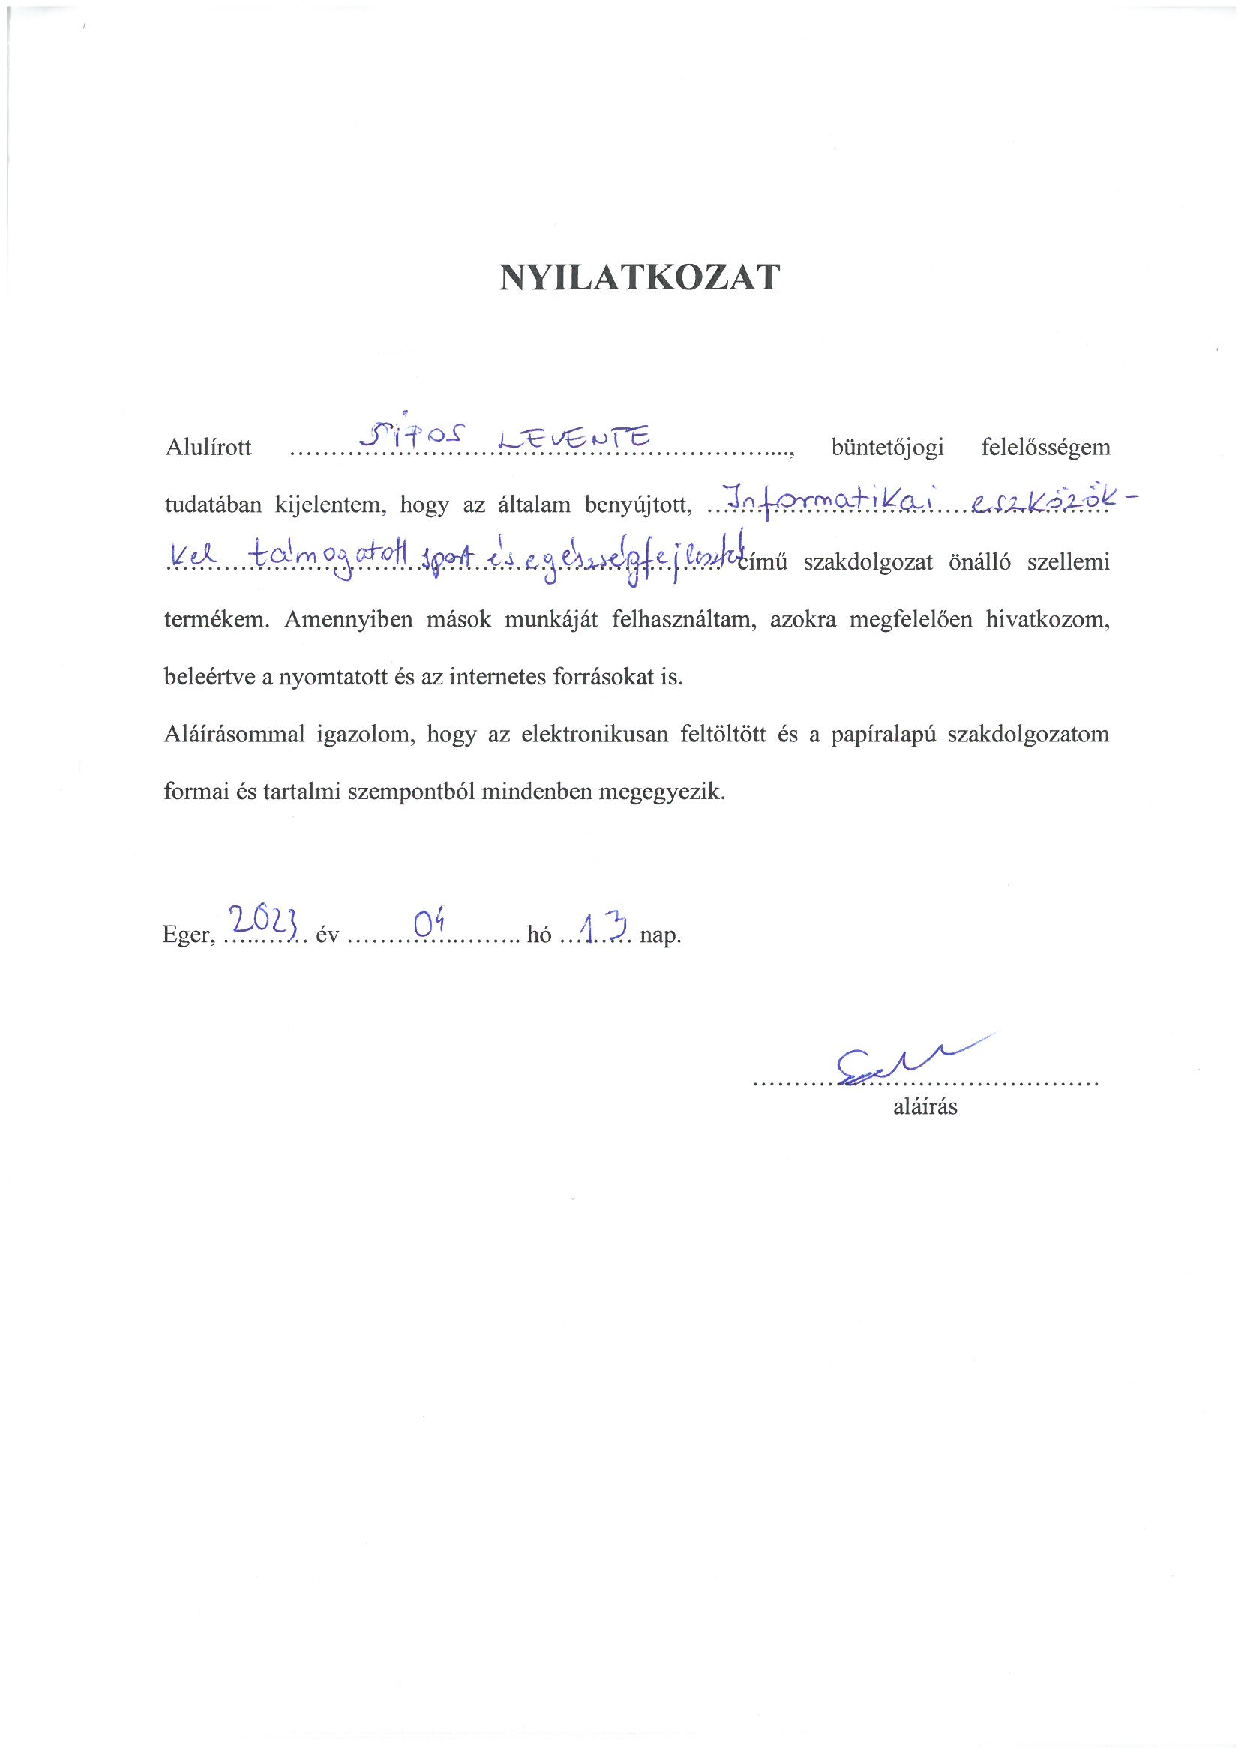
\includepdf{nyilatkozat.pdf}

	\bibliographystyle{IEEEtran}
	\bibliography{references}
	\begin{comment}
		1.Alapötlet, Projekt célja, és hatásai az oktatásra/egézségügyre.
				Miért jó a projekt amit csinálunk?
				Somodi László által kapottak megemlítése
		2.A Winformos projekt
				milyen eszközöket lehet irányítani vele(mire jók)
				panelek külön-külön mit csinálnak
				hogyan kommunikál a Delphi-vel (Bence projektje, megemlítés)
		3. Alacsonyabbszintű komponensek/Imperatív és oop közti kommunikáció(Bence)
				Hangvezérlés
				Színek
				Nyilak
				4 || 8 eszközös megoldások
		4. Projekt tényleges használata, felmérések, és vélemények.
				Gondolatok és meglátások //akár lehet egyel előbb is
	\end{comment}
	% Aláírt, szkennelt nyilatkozat beillesztése a szakdolgozat végére

	\listoffigures
	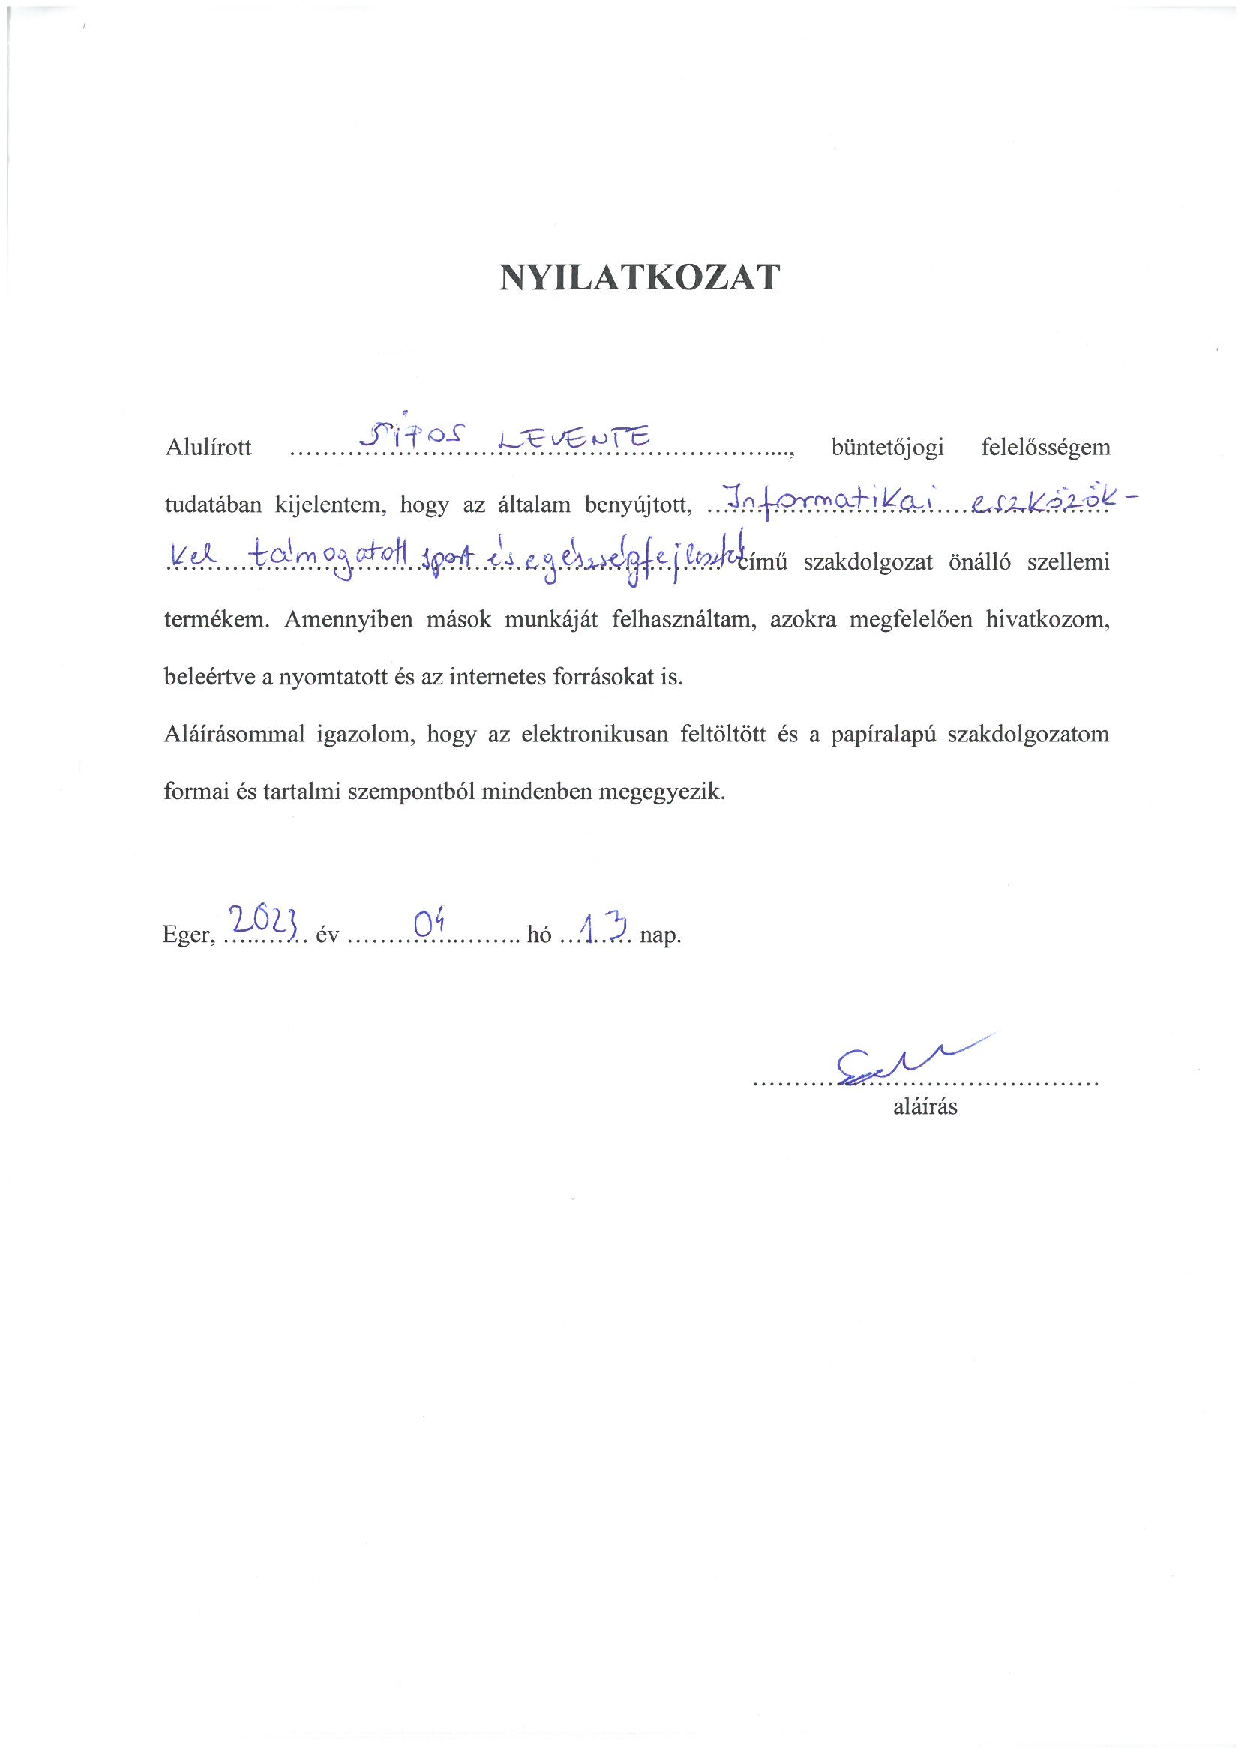
\includepdf{nyilatkozat.pdf}
\end{document}